%%%%%%%%%%%%%%%%%%%%%%%%%%%%%%%%%%%%%%%%%%%%%%%%%%%%%%%%%%%%%%%%%%%%
%%%%%%%%%%%%%%%%%%%%%%%%%%%%%%%%%%%%%%%%%%%%%%%%%%%%%%%%%%%%%%%%%%%%
%%                                                                %%
%% An example for writting your thesis using LaTeX                %%
%% Original version by Luis Costa,  changes by Perttu Puska       %%
%% Support for Swedish added 15092014                             %%
%%                                                                %%
%% This example consists of the files                             %%
%%         thesistemplate.tex (versio 2.01)                       %%
%%         opinnaytepohja.tex (versio 2.01) (for text in Finnish) %%
%%         aaltothesis.cls (versio 2.01)                          %%
%%         kuva1.eps                                              %%
%%         kuva2.eps                                              %%
%%         kuva1.pdf                                              %%
%%         kuva2.pdf                                              %%
%%                                                                %%
%%                                                                %%
%% Typeset either with                                            %%
%% latex:                                                         %%
%%             $ latex opinnaytepohja                             %%
%%             $ latex opinnaytepohja                             %%
%%                                                                %%
%%   Result is the file opinnayte.dvi, which                      %%
%%   is converted to ps format as follows:                        %%
%%                                                                %%
%%             $ dvips opinnaytepohja -o                          %%
%%                                                                %%
%%   and then to pdf as follows:                                  %%
%%                                                                %%
%%             $ ps2pdf opinnaytepohja.ps                         %%
%%                                                                %%
%% Or                                                             %%
%% pdflatex:                                                      %%
%%             $ pdflatex opinnaytepohja                          %%
%%             $ pdflatex opinnaytepohja                          %%
%%                                                                %%
%%   Result is the file opinnaytepohja.pdf                        %%
%%                                                                %%
%% Explanatory comments in this example begin with                %%
%% the characters %%, and changes that the user can make          %%
%% with the character %                                           %%
%%                                                                %%
%%%%%%%%%%%%%%%%%%%%%%%%%%%%%%%%%%%%%%%%%%%%%%%%%%%%%%%%%%%%%%%%%%%%
%%%%%%%%%%%%%%%%%%%%%%%%%%%%%%%%%%%%%%%%%%%%%%%%%%%%%%%%%%%%%%%%%%%%

%% Uncomment one of these:
%% the 1st when using pdflatex, which directly typesets your document in
%% pdf (use jpg or pdf figures), or
%% the 2nd when producing a ps file (use eps figures, don't use ps figures!).
\documentclass[english,12pt,a4paper,pdftex,elec,utf8]{aaltothesis}
%\documentclass[english,12pt,a4paper,dvips]{aaltothesis}

%% To the \documentclass above
%% specify your school: arts, biz, chem, elec, eng, sci
%% specify the character encoding scheme used by your editor: utf8, latin1

%% Use one of these if you write in Finnish (see the Finnish template):
%%
%\documentclass[finnish,12pt,a4paper,pdftex,elec,utf8]{aaltothesis}
%\documentclass[finnish,12pt,a4paper,dvips]{aaltothesis}
\usepackage[super]{nth}
\usepackage{graphicx}
\graphicspath{ {images/} }
\usepackage{listings}
\usepackage{minted}
\usepackage{float}
\usepackage{svg}

\usepackage{booktabs}
\usepackage{multirow}

%% Use this if you write hard core mathematics, these are usually needed
\usepackage{amsfonts,amssymb,amsbsy}


%% Use the macros in this package to change how the hyperref package below 
%% typesets its hypertext -- hyperlink colour, font, etc. See the package
%% documentation. It also defines the \url macro, so use the package when 
%% not using the hyperref package.
%%
%\usepackage{url}

%% Use this if you want to get links and nice output. Works well with pdflatex.
\usepackage{hyperref}
\hypersetup{pdfpagemode=UseNone, pdfstartview=FitH,
  colorlinks=true,urlcolor=red,linkcolor=blue,citecolor=black,
  pdftitle={Default Title, Modify},pdfauthor={Your Name},
  pdfkeywords={Modify keywords}}


%% All that is printed on paper starts here
\begin{document}

%% Change the school field to specify your school if the automatically 
%% set name is wrong
% \university{aalto-yliopisto}
\university{aalto University}
% \school{Sähkötekniikan korkeakoulu}
\school{School of Electrical Engineering}

%% Only for B.Sc. thesis: Choose your degree programme. 
%\degreeprogram{Electronics and electrical engineering}
%%

%% ONLY FOR M.Sc. AND LICENTIATE THESIS: Specify your department,
%% professorship and professorship code. 
%%
\department{Department of Radio Science and Technology}
\professorship{Space Science and Technology}
%%

%% Valitse yksi näistä kolmesta
%%
%% Choose one of these:
%\univdegree{BSc}
\univdegree{MSc}
%\univdegree{Lic}

%% Your own name (should be self explanatory...)
\author{Juha-Matti Lukkari}

%% Your thesis title comes here and again before a possible abstract in
%% Finnish or Swedish . If the title is very long and latex does an
%% unsatisfactory job of breaking the lines, you will have to force a
%% linebreak with the \\ control character. 
%% Do not hyphenate titles.
%% 
\thesistitle{Automated functional system testing of Suomi 100 satellite}

\place{Espoo}

%% For B.Sc. thesis use the date when you present your thesis. 
%% 
%% Kandidaatintyön päivämäärä on sen esityspäivämäärä! 
\date{16.1.2015}

%% B.Sc. or M.Sc. thesis supervisor 
%% Note the "\" after the comma. This forces the following space to be 
%% a normal interword space, not the space that starts a new sentence. 
%% This is done because the fullstop isn't the end of the sentence that
%% should be followed by a slightly longer space but is to be followed
%% by a regular space.
%%
\supervisor{Prof.\ Esa Kallio} 

%% B.Sc. or M.Sc. thesis advisors(s). You can give upto two advisors in
%% this template. Check with your supervisor how many official advisors
%% you can have.
%%
%\advisor{Prof.\ Pirjo Professori}
\advisor{D.Sc.\ (Tech.) Antti Kestilä}
\advisor{D.Sc.\ (Tech.) Juha Itkonen}

%% Aalto logo: syntax:
%% \uselogo{aaltoRed|aaltoBlue|aaltoYellow|aaltoGray|aaltoGrayScale}{?|!|''}
%%
%% Logo language is set to be the same as the document language.
%% Logon kieli on sama kuin dokumentin kieli
%%
\uselogo{aaltoRed}{''}

%% Create the coverpage
%%
\makecoverpage


%% Note that when writting your master's thesis in English, place
%% the English abstract first followed by the possible Finnish abstract

%% English abstract.
%% All the information required in the abstract (your name, thesis title, etc.)
%% is used as specified above.
%% Specify keywords
%%
%% Kaikki tiivistelmässä tarvittava tieto (nimesi, työnnimi, jne.) käytetään
%% niin kuin se on yllä määritelty.
%% Avainsanat
%%
\keywords{For keywords choose concepts that are central to your thesis}
%% Abstract text
\begin{abstractpage}[english]
 Large portion of launched Cubesats have failed early on their missions. Complete lack or inadequate system level functional testing of the satellites has been thought of being one large contributor to these failures according to some research done on the statistical data available about Cubesats. This thesis investigates potential solutions to mitigating these issues by the use of free open-source automated test framework. Presenting how we can do system level testing of Cubesats and what kind of tests could be done.

  Your abstract in English. Try to keep the abstract short; approximately 
  100 words should be enough. The abstract explains your research topic, 
  the methods you have used, and the results you obtained.  
  Your abstract in English. Try to keep the abstract short; approximately 
  100 words should be enough. The abstract explains your research topic, 
  the methods you have used, and the results you obtained.  
\end{abstractpage}

%% Force a new page so that the possible English abstract starts on a new page
%%
%% Pakotetaan uusi sivu varmuuden vuoksi, jotta 
%% mahdollinen suomenkielinen ja englanninkielinen tiivistelmä
%% eivät tule vahingossakaan samalle sivulle
\newpage
%
%% Abstract in Finnish.  Delete if you don't need it. 
\thesistitle{Automatisoitu Suomi 100 satelliitin funktionaalinen systeemitestaus}
\advisor{Prof Esa Kallio}
\degreeprogram{Electronics and electrical engineering}
\department{Radiotieteen ja -tekniikan laitos}
\professorship{Avaruus tiede ja tekniikka}
%% Avainsanat
\keywords{Vastus, Resistanssi,\\ Lämpötila}
%% Tiivistelmän tekstiosa
\begin{abstractpage}[finnish]
  Tiivistelmässä on lyhyt selvitys (noin 100 sanaa)
  kirjoituksen tärkeimmästä sisällöstä: mitä ja miten on tutkittu,
  sekä mitä tuloksia on saatu. 
  Tiivistelmässä on lyhyt selvitys (noin 100 sanaa)
  kirjoituksen tärkeimmästä sisällöstä: mitä ja miten on tutkittu,
  sekä mitä tuloksia on saatu. 

  Tiivistelmässä on lyhyt selvitys (noin 100 sanaa)
  kirjoituksen tärkeimmästä sisällöstä: mitä ja miten on tutkittu,
  sekä mitä tuloksia on saatu. 
  Tiivistelmässä on lyhyt selvitys (noin 100 sanaa)
  kirjoituksen tärkeimmästä sisällöstä: mitä ja miten on tutkittu,
  sekä mitä tuloksia on saatu. 
  Tiivistelmässä on lyhyt selvitys (noin 100 sanaa)
  kirjoituksen tärkeimmästä sisällöstä: mitä ja miten on tutkittu,
  sekä mitä tuloksia on saatu. 
\end{abstractpage}

%% Force new page so that the Swedish abstract starts from a new page
\newpage
%
%% Swedish abstract. Delete if you don't need it. 
%% 
\thesistitle{Arbetets titel}
\advisor{TkD Olli Ohjaaja} %
\degreeprogram{Electronik och electroteknik}
\department{Institutionen för radiovetenskap och -teknik}%
\professorship{Kretsteori}  %
%% Abstract keywords
\keywords{Nyckelord p\aa{} svenska,\\ Temperatur}
%% Abstract text
\begin{abstractpage}[swedish]
 Sammandrag p\aa{} svenska.
 Try to keep the abstract short, approximately 
 100 words should be enough. Abstract explains your research topic, 
 the methods you have used, and the results you obtained.  
\end{abstractpage}

%% Preface
%%
%% Esipuhe 
\mysection{Preface}
%\mysection{Esipuhe}
I want to thank Professor Esa Kallio
and my instructors Antti Kestilä and Juha Itkonen for their 
good guidance.\\

\vspace{5cm}
Otaniemi, 16.1.2015

\vspace{5mm}
{\hfill Eddie E.\ A.\ Engineer \hspace{1cm}}

%% Force new page after preface
%%
%% Pakotetaan varmuuden vuoksi esipuheen jälkeinen osa
%% alkamaan uudelta sivulta
\newpage


%% Table of contents. 
\thesistableofcontents


%% Symbols and abbreviations
\mysection{Abbreviations}

%\subsection*{Symbols}

%\begin{tabular}{ll}
%$\mathbf{B}$  & magnetic flux density  \\
%$c$              & speed of light in vacuum $\approx 3\times10^8$ [m/s]\\
%$\omega_{\mathrm{D}}$    & Debye frequency \\
%$\omega_{\mathrm{latt}}$ & average phonon frequency of lattice \\
%$\uparrow$       & electron spin direction up\\
%$\downarrow$     & electron spin direction down
%\end{tabular}

%\subsection*{Operators}

%\begin{tabular}{ll}
%$\nabla \times \mathbf{A}$              & curl of vectorin $\mathbf{A}$\\
%$\displaystyle\frac{\mbox{d}}{\mbox{d} t}$ & derivative with respect to 
%variable $t$\\[3mm]
%$\displaystyle\frac{\partial}{\partial t}$  & partial derivative with respect 
%to variable $t$ \\[3mm]
%$\sum_i $                       & sum over index $i$\\
%$\mathbf{A} \cdot \mathbf{B}$    & dot product of vectors $\mathbf{A}$ and 
%$\mathbf{B}$
%\end{tabular}

%\subsection*{Abbreviations}

\begin{tabular}{ll}
GPS 	& Global Positioning System \\
COTS 	& Commercial-off-the-self \\
Cal Poly	& California Pylotechnic State University \\
1U 		& 1 Unit CubeSat \\
P-POD	& Poly Picosatellite Orbital Deployer \\
PCB 	& Printed Circuit Board \\
EPS      & Electric Power System \\
OBC 	& On-Board Computer \\
COMM 	& Communication System \\
ADCS 	& Attitude Determination and Control System \\
DOA 	& Dead On Arrival \\
CFD 	& CubeSat Failure Database \\
NASA 	& National Aeronautics and Space Administration \\
SUT 	& System Under Test \\
ESA 	& European Space Agency \\
TLYF 	& Test Like You Fly \\
CONOPS 	& Operation Concept Document \\
RF 		& Radiofrequency \\
UHF 	& Ulta-High Frequency \\
AM 		& Amplitude Modulated \\
MCU 	& Microcontroller Unit \\
RISC 	& Reduced Instruction Set Computer \\
I2C 	& Inter-Integrated Circuit \\
CAN 	& Controller Area Network \\
GPIO 	& General Purpose Input-Output \\
SDRAM 	& Synchronous Dynamic Random Access Memory \\
PA	 	& Power Amplifier \\
LNA 	& Low-noise Amplifier \\
CMOS 	& Complementary Metal Oxide Semiconductor \\
IC 		& Integrated Circuit \\
FM 		& Frequency Modulated \\
CSP 	& CubeSat Space Protocol \\
HK 		& Housekeeping \\
GOSH 	& GomSpace Shell \\
FTP 	& File Transfer Protocol \\
RTOS 	& Real-time Operating System \\
API 	& Application Programming Interface \\
Stdin 	& Standard Input Stream \\
Stdout 	& Standard Output Stream \\
SDR		& Software Defined Radio \\
FFT 	& Fast Fourier Transform \\
CI/CD 	& Continuous Integration/Continuous Development

\end{tabular}


%% Tweaks the page numbering to meet the requirement of the thesis format:
%% Begin the pagenumbering in Arabian numerals (and leave the first page
%% of the text body empty, see \thispagestyle{empty} below).
%% Additionally, force the actual text to begin on a new page with the 
%% \clearpage command.
%% \clearpage is similar to \newpage, but it also flushes the floats (figures
%% and tables).
%% There is no need to change these
%%
\cleardoublepage
\storeinipagenumber
\pagenumbering{arabic}
\setcounter{page}{1}


%% Text body begins. Note that since the text body
%% is mostly in Finnish the majority of comments are
%% also in Finnish after this point. There is no point in explaining
%% Finnish-language specific thesis conventions in English. Someday 
%% this text will possibly be translated to English.
%%
\section{Introduction}
%\section{Introduction}

%% Ensimm\"ainen sivu tyhj\"aksi
%% 
%% Leave first page empty
\thispagestyle{empty}
\subsection{Increasing interest in space}
Since 1950s, mankind has ever increasingly started to set its foot into space \cite{aftersputnik}. Nations, industries, businesses, militaries, universities and even private entrepreneurs have sought out to benefit from the opportunities that space offers \cite{aftersputnik, rocketeers, Swart1}. Great advancements have been made in technology and science to propel this endeavour even further \cite{aftersputnik}. Examples of such leaps in techology include sending first human into space in 1957, Moon landings in 1969, sending of probes into other planets in the Solar System like Mars and most recenlty getting the first images of Pluto in a flyby mission in 2013 \cite{aftersputnik, pluto}. Use of space technology has also entered into household items through for example the use of the \textit{Global Positioning System} (GPS) satellite network in mobile phones, cars, and so forth \cite{satcommunications}. People and industries have began increasingly to be reliant on space borne technologies and devices \cite{satcommunications}.\par
Since the end of the 1990s new inventions have brought design and manufacturing of these technologies relatively closer to everyday people, away from the assembly sites of large nations and large organizations into laboratories run for example by university students. Advancements leading to this can be attributed to the space industry cathcing up with the advancements of electronics as well as cheap launch opportunities coming available. More concretely, development of the \textit{CubeSat} nanosatellite concept in 1999 in CalTech has in recent years brought about hundreds of new satellite developers and hundreds of new space missions based on this nanosatellite concept. \cite{Swart1, Swart2016}\par 
These satellites typically are relatively small and usually use commercial off-the-self (COTS) components, yet are still capable to operate in space around Earth. Cubesats have in recent years emerged as a new viable platform for carrying out space missions. Due to their small size the launch costs are smaller and their use of COTS components makes them relatively fast and relatively cheap to design and manufacture.  Several companies have taken interest into the concept and other organizations (like US military) have shown interest into them as well \cite{cds}. In addition, Finnish government recently passed a new law regarding space and is pursuing to create a new industry of space technology related companies in Finland \cite{filaw}. The first Cubesats built in Finland in Aalto University have even created new space companies which are building their own satellites to be launched into space, like \textit{Iceye} for example  \cite{iceye}. Nonetheless, usually most of these satellites have been produced by Universities and over 600 Cubesats have already been launched in total since 2000 \cite{Swart2017kalvo}. The trend seems to be so that more and more CubeSat missions are to come and they are starting to take a clear share of the space industry market \cite{SpaceWorks2017}. Already in 2014, approximately half of the flown space missions in that year were CubeSats \cite{Swart2016}.\par 
\subsection{Substantial proportion of failures in CubeSat missions}
Even though the CubeSat concept has rapidly created large amount of new space missions, large portion of those launched missions have ended in failure due to various reasons. Several surveys done in recent years have found a failure rate of 40 \% for new CubeSat missions. Yet, if the satellites were manufactured by teams with earlier experience in space missions, the failure rates were considerably lower. Suggestions have been made in these surveys that the missions that have failed haven't done proper functional testing on ground on a system level or that such testing has been missing completely. As an example, research done by Swartwout in 2013 into statistical data of first 100 flown Cubesats discovered that over 40 \% of Cubesat missions ended in failure. This research suggests that majority of these failures could be attributed to inadequate testing of the satellite in a flight-equivalent state on ground. It was believed that functional testing of the whole integrated satellite system has been lacking completely or done in a very limited sense. This allegation could been made at least for those missions where the satellite was never contacted from the ground station after the launch, as many of the failures in these missions were attributed to failures in system integration. Such as the solar panels not being properly connected, insufficient power generated for the transmitter, unrecoverable processor errors and so forth. \cite{Swart1, Swart2016, Swart2015, Langer}\par
Some examples of early life failures include Aalto-2 satellite, the first Finnish satellite flown in space [source]. Though the concept of Cubesats shows promise, there are still some challenges for the concept to become a truly reliable alternative approach for scientific and commercial missions alike as opposed to the more traditional time and resources consuming approaches in space mission development \cite{Swart1}.\par 
\subsection{Suomi100 Cubesat} 
The satellite involved in our research is called \textit{Suomi100} which is a one unit Cubesat. The project was conceived in the interest of celebrating Finland's 100 years of independence. Mission of satellite is to take images of Finland from space and to measure different radio signals present in the ionosphere. An artistic presentation can be seen in Figure \ref{s100intro} below.
\begin{figure}[!h]
\centering
\includegraphics[scale=0.2]{s100_orbit}
\caption{Depiction of Suomi100 satellite in space. Courtesy of Jari Mäkinen. \cite{s100blogi}}
\label{s100intro}
\end{figure} 
\subsection{Research purpose and goals}
The aim of this thesis is to investigate \textit{how to carry out
functional system testing in order to improve CubeSat reliability}. Further, we wish to automate the testing and to do it systematically, just as the verification tests for example for mechanical stress are done systematically in an automated fashion. So too it would be preferable that the functional system tests could be done automatically in a systematic manner.\par 
On the technology point of view, the goal will be obtained by developing new generic Python library and test suites which can be used in \textit{Robot Framework} \cite{robotmain} along with appropriate test setups.\par 
\subsection{Main questions and problems}
The main problem is the unreliability of Cubesats, which the thesis tries to partly solve from the standpoint of system integration testing. Could this type of testing detect unrecoverable failures in the satellite operation and system integration and could we in addition verify that the satellite meets out its functional requirements?
\subsection{Outlining the scope of research}
We wish to study the use of one industry-proven automated acceptance framework to carry out the automated functional testing on Suomi100 and to investigate the use of industry-proven testing philosophies and methodologies into functional system testing with the satellite.\par
In conjunction with the space industry test methodologies, we attempt to some degree simulate the environment related to functional operations of the satellite. In addition, the simulation has to take into account the relatively small funds of an university led project.\par
%% Esimerkki luettelosta. Lyhyt ajatusviiva on k\"ayt\"oss\"a
%% luettelossa, ja se on pituudeltaan
%% en dash. Merkit\"a\"an latex-koodissa --. 




%% Opinn\"aytteess\"a jokainen osa alkaa uudelta sivulta, joten \clearpage
%%
%% In a thesis, every section starts a new page, hence \clearpage
\clearpage

\section{Background}
%\section{Aikaisempi tutkimus}
\subsection{Cubesat failures}
The CubeSat project was started in 1999 in California Polytechnic State University (Cal Poly) \cite{cds}. Over 100 universities and other organisations have since contributed to the project. The purpose of the project is to provide a standard for design of picosatellites in order to decrease development costs and to make accessability to space easier \cite{cds}. In fact, number of launched CubeSats has increased quite dramatically over the past few years \cite{Swart2016} and it has been estimated that the number of CubeSat missions will increase in the coming years \cite{SpaceWorks2017}. Yet, large portion of these missions have failed due to various reasons \cite{Swart1, Swart2016, Swart2015}. With only an average of 20 \% of missions being able to complete the full mission envisioned for them \cite{Swart2016}. \par 
\subsubsection{CubeSat satellite}
The CubeSat project defines a CubeSat to be a picosatellite with dimensions of ${10 * 10 * 10 cm^3}$ and with a mass up to 1.33 kg \cite{cds}. Satellite of this size is considered to be \textit{one unit} (1U) CubeSat. These units can be stacked together to form larger CubeSats, with some satellites consisting even of 12 units. Three units seems to statistically be the preferred size for a CubeSat \cite{Swart2016}. \par
Another important part of the concept is the \textit{Poly Picosatellite Orbital Deployer} (P-POD), which is a Cal Poly’s standardized CubeSat deployment system \cite{cds}. This deployment system is integrated to the launch vehicle and the springs in the system release the picosatellites into space \cite{cds}. Usually a launch vehicle carries some primary payload, which is much larger than the CubeSats \cite{nasacubesat1}. If an extra weight can be launched along the main payload, then the deployment pods with the CubeSats are integrated into the launch vehicle as secondary payloads \cite{nasacubesat1}. \par 
Though these picosatellites are considerably smaller than most of the "traditional" satellites, they nonetheless are able to perform the regular operations of a satellite \cite{openorbiter}. As the classification, \textit{picosatellite} defines, CubeSats are satellites in miniature size. Even though smaller, the same general class of subsystems are part of CubeSats as they are part of larger satellites \cite{openorbiter}. Subsystems containing electronics usually follow \textit{PC/104} standard which defines form factor and computer bus \cite{reliabilitycubesatelbus}. A single subsystem in a CubeSat can fit into one \textit{Printed Circuit Board} (PCB) following the PC/104 standard \cite{reliabilitycubesatelbus}.\par
Figure \ref{s100cad} illustrates the internal structure of Suomi100 CubeSat and the different subsystems that are integrated into the satellite.\par 
\begin{figure}[!h]
\centering
\includegraphics[scale=0.2]{s100cad}
\caption{Depiction of Suomi100 satellite subsystems. Courtesy of Aalto University. \cite{s100blogi}}
\label{s100cad}
\end{figure}  
From this figure we can identify five subsystems that are common to all satellites. Power to the satellite is produced by the \textit{Electric Power System} (EPS) and this subsystem consists of the solar panels and batteries in the satellite. The subsystem usually in addition has some power regulation and power distribution features along some features for reliability. \cite{spacesystemsengineering}\par 
The central computer of the satellite is called \textit{On-Board Computer} (OBC) and the task of this subsystem is to orchestrate the operation of all the other subsystems. In addition, the processing of commands received from the ground station and the routing of them to the appropriate subsystem is the task of the OBC. \cite{spacesystemsengineering} \par 
The \textit{Communication system} (COMM) is responsible for communication with the ground station. This subsystem usually has a computer of its own for processing the received radio signals. The antennas are also part of this system \cite{spacesystemsengineering}. \par
The proper orientation of the satellite is controlled by \textit{Attitude Determination and Control System} (ADCS). For CubeSats, the orientation can be controlled either by mechanical reaction wheels, magnetorquers or by some other methods. The purpose of this system is to keep track of the orientation of the satellite and to change it according to commands received from ground station. \cite{spacesystemsengineering}\par 
In addition to these subsystems, \textit{Support Structure} forms the subsystem which integrates all of the subsystems into a single mechanical structure \cite{spacesystemsengineering}. The CubeSat standard defines the dimensions and materials for the support structure \cite{cds}.    
\subsubsection{Failure rates of CubeSats}
Over 600 Cubesats have been launched as of 2017 \cite{Swart2017kalvo}. Some studies in recent years have been carried out to investigate the statistics of flown Cubesat missions. These studies looked for the percentage of failed missions and which subsystems contributed to each failure. Out of these failures, the amount of \textit{dead on arrival} (DOA) missions where the satellite was never contacted from space were also identified. Most active contributor to this topic has been Michael Swartwout and the representation of statistics of CubeSat failures in this thesis is mainly based on his work \cite{Swart1, Swart2016, Swart2015}, as not too many papers have yet been published regarding this issue.\par 
A study titled \textit{The First One hundred CubeSats: A Statistical Look} and published in 2013 was one of the first papers to analyze the statistical data of flown CubeSats. Out of the first 100 CubeSat missions investigated between years 2000-2012, a total of 34 had failed. Out of these failures, third were never contacted after they were released into space (DOA cases). Since then, many CubeSats have flown with varying degree of success \cite{Swart2016}. Figure \ref{100first} shows mission statistics for all CubeSats flown until 2017 \cite{csdatabase}. \par
\begin{figure}[h!]
\centering
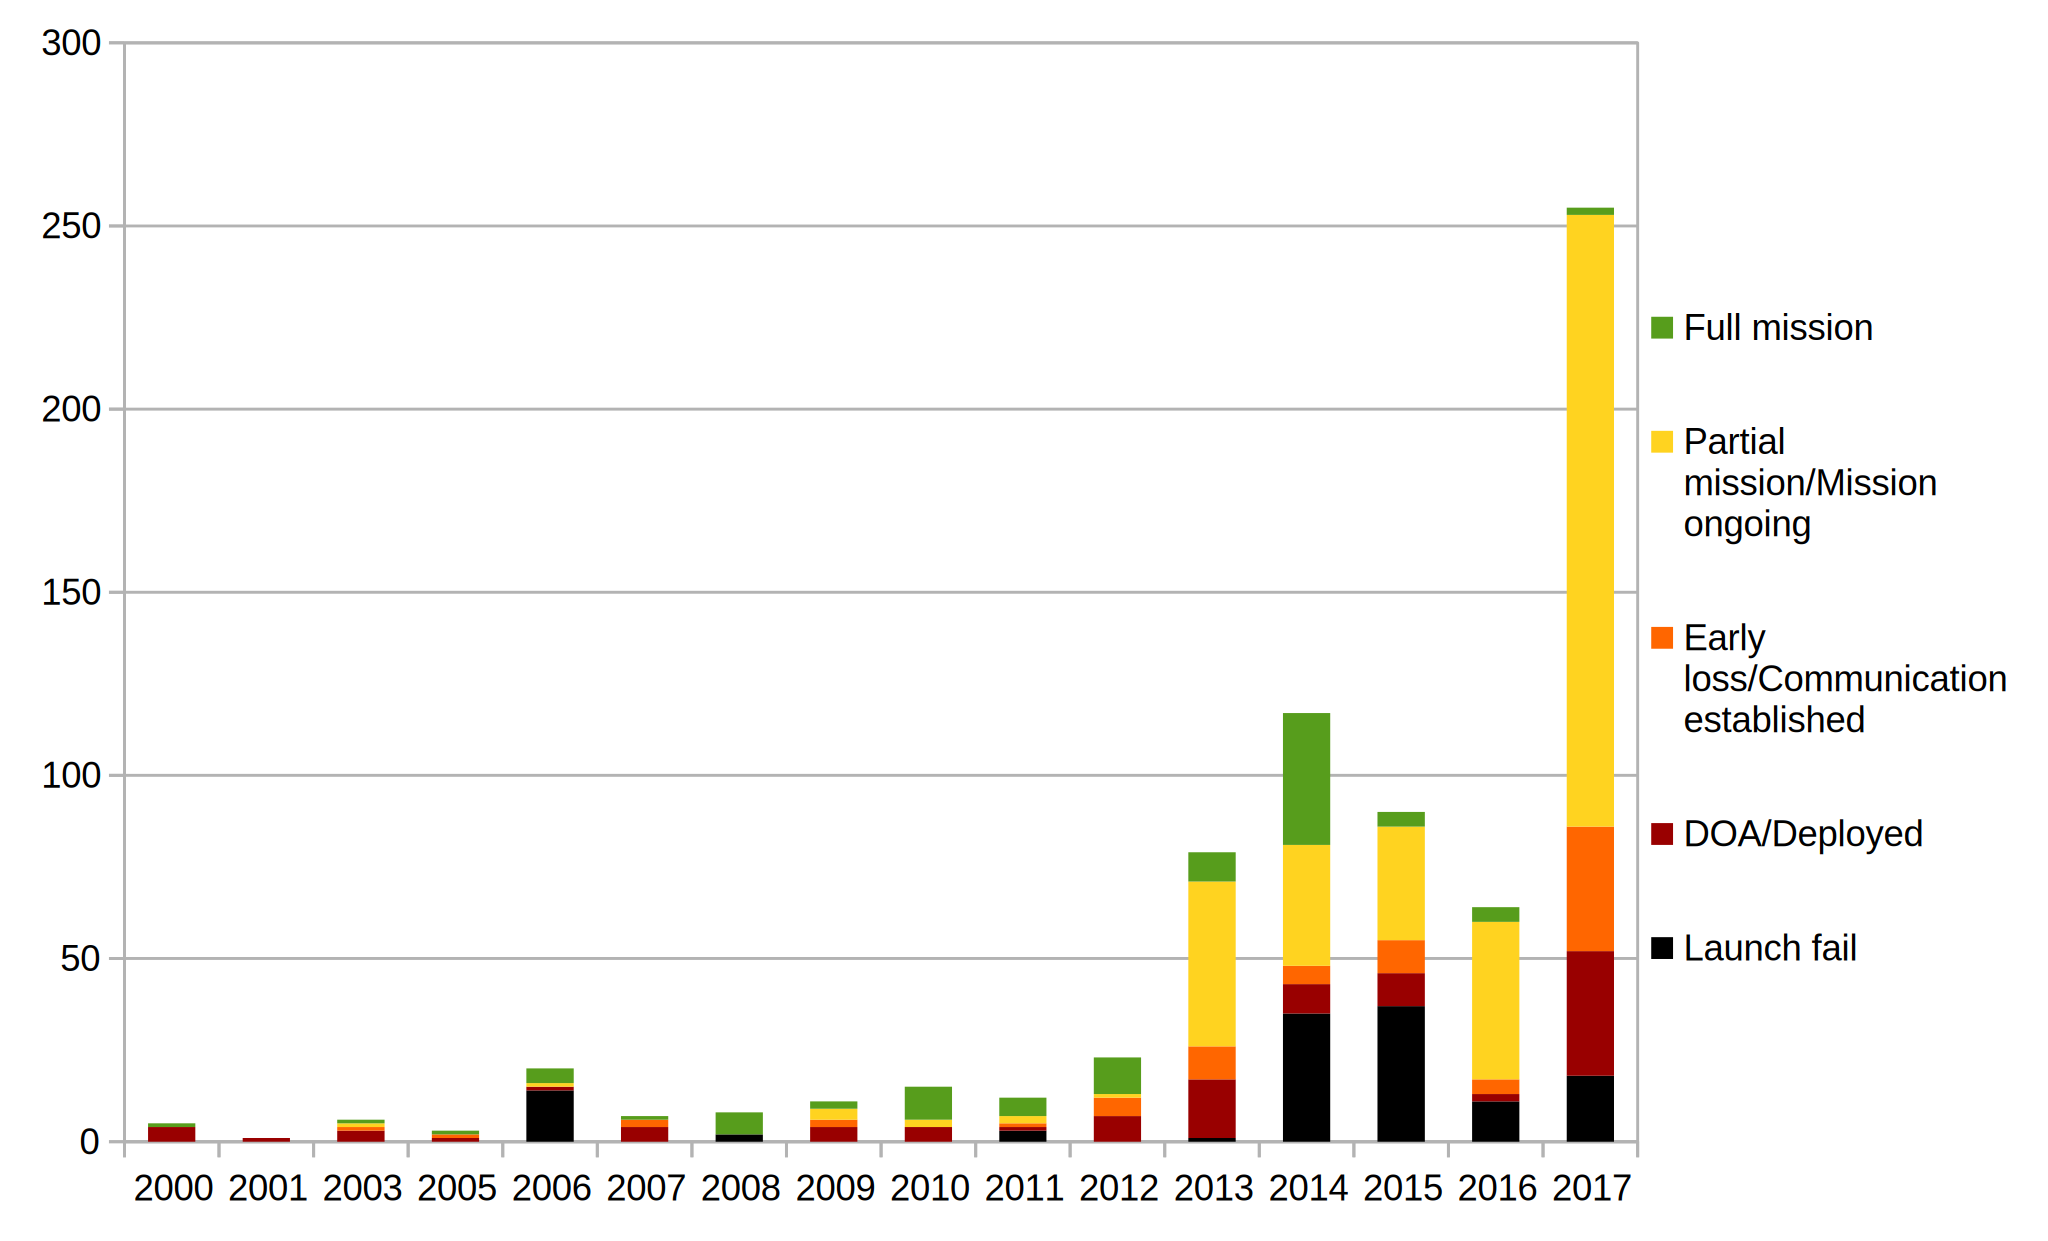
\includegraphics[scale=0.6]{cfdnew}
\caption{Mission statistics for CubeSats flown until 2017. \cite{csdatabase}}
\label{100first}
\end{figure} 
In order to break down and investigate the statistics, Swartwout has been continuing yearly to publish papers about the statistics of CubeSat failures, as new missions are flown each year \cite{Swart2016, Swart2015}. In these papers Swartwout has included statistics about other secondary payloads as well, though majority of secondary payloads have been CubeSats. A study published in 2016 titled \textit{Secondary Spacecraft in 2016:
Why Some Succeed (And Too Many Do Not)} identified out of all CubeSats flown between 2000-2015 that reached orbit 21 \% DOA cases and 9.8 \% cases where the spacecraft was lost early in its life, meaning that communication with the satellite was established but no primary operations could have been executed. When breaking down the statistics to categories based on the type of satellite and mission developer (new University teams, traditional contractors, experienced University and government teams, constellations), it was found that for the new University teams flying their first satellite, the failure rates were as follows: 44.1 \% DOA, 16.2 \% early loss and 16.2 \% mission success. On the other hand, for the CubeSats built by traditional contractors with established practices for integration and testing the numbers were: 6.3 \% DOA and 6.3 \% early loss. On the other hand, when the new University teams educated by their first failure flew their second satellite, the rates for DOA failures halved. \cite{Swart2016, Swart2015}\par 
Below Figure \ref{hobbyistflown2015pic} shows the statistics of failures for CubeSats between 2000-2015 flown by new University teams sending their first satellite, excluding those missions where the satellite was lost due to launch failure.\par 
\begin{figure}[h!]
\centering
\includegraphics[scale=0.5]{university2015}
%\includesvg[]{images/university2015svg}
\caption{Statistics for CubeSats flown between 2000-2015 that were constructed by University teams without prior experience for satellite construction. \cite{Swart2016}}
\label{hobbyistflown2015pic}
\end{figure} 
For contrast, same statistics for CubeSats built by traditional contractors is shown in figure \ref{tradiotionalflown2015pic} below. \par
\begin{figure}[h!]
\centering
\includegraphics[scale=0.5]{traditional2015}
\caption{Statistics for CubeSats flown between 2000-2015 that were constructed by traditional contractors with extensive experience of satellite construction. \cite{Swart2016}}
\label{tradiotionalflown2015pic}
\end{figure} 
\subsubsection{Contribution of different subsystems to satellite failures}
Some study has been carried out by Swartwout in one of the aforementioned papers to investigate the contribution of different subsystems in CubeSat failures. In the paper \textit{The First One hundred CubeSats: A Statistical Look}, the subsystems that were thought of been the cause of the failure were identified as follows: a configuration or interface failure between communications hardware (27\%), the power subsystem (14\%) and the flight processor (6\%), or COMM, EPS and OBC subsystem. A failure in a subsystem means in this context that the whole satellite is lost due to the failure. A failure in the OBC can mean for example that the processor doesn't reboot anymore or gets unrecoverable stuck in some way. For EPS the error can mean for example that power is not being transferred to the satellite from the solar panels and for the failure in COMM subsystem it can mean for example that there is insufficient power for the antennas to close the link with the ground station.  \cite{Swart1}\par
Based on the satellite developers believes about causes of failures, another study was carried out by Langer et al. in 2014 \cite{Langer} to investigate in more detail the contribution of different subsystems in CubeSat failures. This study by Langer also used statistical data of CubeSat failures obtained from CubeSat Failure Database (CFD), at that point comprising data about 178 CubeSat missions. With this data a reliability estimate for different subsystems was calculated using Kaplan-Meier estimator for nonparametric and parametric analysis. In addition, a parametric model for total CubeSat satellite reliability was devised. Figure \ref{subsystemfailures} below depicts the subsystem contributions to satellite failures for the 178 CubeSat missions. Three main subsystems causing failures were identified to be in order: EPS, OBC and communication systems, in accordance with Swartwout research, but with different percentages as EPS being the main contributor to failures \cite{Swart1, Langer}. \par
\begin{figure}[h!]
\centering
\includegraphics[scale=0.5]{subsystemmerge}
\caption{Developers believes on the contribution of different subsystems to satellite failure. From left to right the charts present failure contribution data for 0, 30 and 90 days after launch. \cite{Langer}}
\label{subsystemfailures}
\end{figure}  
The statistical data gathered from questionnaires sent to 987 satellite developers (with 113 returned fully completed) showed that there was a belief that within the first six months there was a 50 \% change that the satellite fails. Yet, the developer's belief seems to be too optimistic when compared to the data gathered from CFD. Nonetheless, from largest to smallest probability for causing system failure the main subsystems were identified in the order COMM, EPS and OBC.\cite{Langer}\par
\subsubsection{Needs for the system level functional testing}
The aforementioned studies made some anecdotal guesses to what could have contributed to the failures in the satellites so that the missions failed either partially or completely. The current data doesn't clearly prove these guesses, it has been believed by Swartwout and others that system level functional testing of the satellites has been lacking completely or has been inadequate \cite{Swart1, Swart2016, Swart2015, Langer}. \par
Based on his study in 2013 \cite{Swart1}, Swartwout came to a strong belief that the critical failures in the subsystems were caused by poor functional integration. Notably, out of first 30 identified DOA cases, 24 were CubeSats made by university teams. In addition, based on his discussions with project managers and faculty leaders it was noted that university teams constructing CubeSats have the misconception that the satellite works as expected the first time it is assemled together and thus no system level functional testing is performed. In this paper it was believed that operational tests demonstrating "a day in the life of the satellite" would be just as necessary as the vibrational tests to certify a CubeSat ready for launch. In addition, testing of recovery from resets, power management, startup sequences etc. would be important operations of the satellite to test. \cite{Swart1} \par
In later papers Swartwout has been less reluctant to make these claims directly, yet still identifying the large number of failed CubeSat missions coming from university-led satellite teams \cite{Swart2016, Swart2015}. As an example, the ORS-3 mission flown in 2013 consisted of 28 secondary payloads and out of these 13 were done by new university teams flying their first satellite and 15 were done by traditional contractors \cite{Swart2016}. While almost all (11 out of 13) of the university constructed CubeSats failed, only one CubeSat built by a traditional contractor failed. Furthermore, all of these satellites had to go through the same vibrational and thermal tests and in addition were subject to mission readiness reviews by the \textit{National Aeronautics and Space Administration} (NASA) and/or Department of Defense of United States. Thus, some practices applied by the experienced contractors in satellite development were quite possibly missing from the university built CubeSats.\par
In addition, David Voss of the Air Force Research Lab speaking more recently in the 31st Annual Conference on Small Satellites held at 7th of August 2017 about CubeSat reliability said that based on his experience with student and other small satellite projects, a core set of tests for power, communication and other subsystems would be needed \cite{smallsatconf31}. Furthermore, Michael Johnson, also a participator in the aforementioned conference and chief technologist at NASA's Goddard Space Flight Center has been since 2017 working at NASA on making a reliability iniative to determine the best ways to improve CubeSat reliability \cite{smallsatconf31, ssvi}. He noted though that the goal is not apply the same rigorous assurance procedures used earlier in larger and more expensive spacecrafts, but to design new procedures and keep some of the familiar methods that can be useful. \par 
\subsubsection{Comparison of CubeSat failures to failures with larger spacecrafts}
Besides Cubesats, failures have happened to the more traditional spacecrafts as well. In fact, the history of space industry as a whole is filled with examples of failed missions [source]. In recent years, for example several Mars landers have failed during landing phases of the mission \cite{marsfailures}. As an example, Mars lander \textit{Schiaparelli} crashed on the Martian surface in 2016 when a sensor used to measure distance to the ground read a negative value and shut off its descent thrusters \cite{schiaparelli}.\par
Earlier research about the on-orbit failures was carried out in 2005 \cite{onorbitfailures}. It investigated failures of 129 different spacecrafts between the years 1980 and 2005, before any flown Cubesats, and it noted that though these spacecrafts had gone through intensive testing and used the most recent technologies available, there where still cases where the spacecraft failed early during its mission. The investigation also found that adequate testing on ground could mitigate these failures as it was noted that the early failures could have been caused by inadequate testing and inadequate modeling of the environment where the spacecraft operates in. These conclusions in fact seem to be similar to what some of the surveys done on CubeSat failures indicate. \cite{onorbitfailures} \par
A research conducted in 2008 analyzed the contributions of different subsystems in failures of  1584 satellites that were launched between 1990 and 2008 \cite{satsubsystems}. Solar array deployment and failure in the communication system were the major contributors to satellite failures for satellites that failed before 30 after launch. After much longer operation time, the main subsystems contributing to failures were identified to be the ADCS and COMM. Some similarity to the subsystem failures with CubeSats can be drawn from here, with the communication subsystem and the solar panels playing a crucial role in infant mortality of CubeSats.\par 
Further prove for the need of extensive testing was found after NASA initiated in the 1990s a more streamlined verification strategy based on the best commercial practices, commonly known as \textit{"Faster, Better, Cheaper"} \cite{satverplanning}. This led to poor results with commercial satellites that were launched during that period and a return to the more rigorous specifications and standards was expressed \cite{satverplanning}. In addition, a study conducted during this period in 1999 called \textit{"When Standards and Best Practices Are Ignored"}, found that out of 50 major space system failures 32 \% were related to inadequate verification and test processes \cite{whenstandignored}.\par 
In conclusion, based on the experiences found by traditional space industry, the allegation that many CubeSat failures are due to poor system integration level testing could be correct.\par 
\subsection{General testing practices}
Why do we talk about software testing?
Since 1970s, testing has been considered as a specific branch of software engineering \cite{artofsofttesting, compinspace}. More advanced techniques and methods for testing have been developed over the decades \cite{artofsofttesting}. For example, 
NASA has contributed to the practices used in software testing through its efforts in the Apollo program \cite{compinspace}. \par
First a relevant question, \textit{who do we need to perform testing?} One reason is that humans make errors and often make optimistical assumptions about their work. Another aspect would be to call testing as a method of proving that the system under test works as we want it to work. Just as  a scientist carries out experiments to prove his theory, so too testing is done to prove that the system works as expected. \cite{testingcomplex}\par
Another important aspect of testing is to find defects in the system and to recognize where they exist so that they can be corrected effectively \cite{sularikurssi, artofsofttesting}. A book by Glenford J. Myers titled \textit{The Art of Software Testing}, defines software testing as \textit{"Testing is the process of executing a program with the intent of finding errors"}, which is a general enough definition to contain many aspects of software testing \cite{artofsofttesting}.
\subsubsection{Methods of testing}
Various different methods for software testing exist. So called box approach is one common method for testing. Testing can either be done automatically by some computer run script or manually by a tester who follows a specified test plan. \cite{sularikurssi} Below are some of the testing methods explained in more detail.\par 
\textbf{Black box testing} is done with no knowledge about the internal structure of the \textit{System Under Test} (SUT), which can be a single function of a software or the whole integrated system. A select set of inputs are given to the system and from outputs we see how did the system perform. If the outputs were what we expected, the system passed the test. Black box testing is usually implemented when we are interested in the functionality of our system under test and test cases are designed from the specifications and requirements of the SUT. There exists some philosophy in choosing the right inputs to the system or software. With \textit{exhaustive testing} all possible input combinations are investigated, which usually leads to combinatorial explosion and the testing all of them can for example even take millions of years! \textit{Boundary-value testing} solves this issue by having some logical set of combinations and not all possible ones. Figure \ref{boxfigurespuge} below illustrates black box testing method. \cite{sularikurssi}\par 
\textbf{White box testing} is done with interest about the internal structure of the SUT. Testing of the internal functions rather than the expected functionality is the goal of white box testing and test cases are derived from the code of the SUT. Usually this type of testing is performed at the smaller component or unit level of the system. Figure \ref{boxfigurespuge} below gives an illustration about white box testing. \cite{sularikurssi}\par
\begin{figure}[h!]
\centering
\includegraphics[scale=0.4]{whiteblackbox}
\caption{Black and white box testing methods. [source]}
\label{boxfigurespuge}
\end{figure} 
\subsubsection{Levels of testing}
Testing can be carried out at different levels of the system and at each level we investigate different aspects of the system. Usually testing of an entire software is done by starting from smaller parts and gradually going into larger components of the system. \cite{sularikurssi, testingcomplex}
One can define different levels of testing as follows \cite{sularikurssi, testingcomplex}:\par 
\textbf{Unit testing}\par 
Unit testing is the most basic level of testing. On this level, individual components of a software or system are tested separately. For example, testing the outputs of a given software function is considered a unit test. Usually these tests are written or performed by the person who also wrote that particular part of the software. Black box and white box methods are usually applied for unit tests. \cite{sularikurssi}\par
\textbf{Integration testing}\par 
Integration testing tests the functionality of larger software or system components, consisting usually of several smaller units. With this level of testing we ensure that the smaller units interact with each other properly and that the bigger component itself works properly. Both black box and white box method can be applied to carry out the tests. \cite{sularikurssi}\par
\textbf{System testing}\par 
On this level, testing is done on a complete integrated system to see whether it conforms to the requirements specified for it or not. With this testing we see whether the integrated parts of the system work together and also see how the whole system functions. Black box testing is usually applied at this level. \cite{sularikurssi}\par
\textbf{Acceptance testing}\par 
Acceptance testing is usually performed after the system in question has passed system testing. At this point testing is usually performed by some outside team that wasn't involved in the development of the system or software. This team could mean customers or there could be a separate testing team to ensure the functionality of the product. Blac box testing methods are applied at this level.\par
\subsubsection{Types of testing}
Besides the method and level of testing chosen, there exists multiple different types of testing that can be performed. The most common ones are the following \cite{sularikurssi}:\par
\textbf{Functional testing}\par
Functional testing is performed when we are interested in knowing what the system under test does based on our input to it. Black box testing methods are mostly applied here. Functional testing can be done at all levels of testing.\par 
\textbf{Non-functional testing}\par
Non-functional testing on the other hand is interested in how the SUT operates, rather than what it actually does. Several different testing types can be considered to belong under this, like e.g. performance testing or security testing. Both black and white box methods can be applied to this type of testing.\par 
\textbf{Performance testing}\par
Performance testing is done for the interest of knowning how stabile and responsive the system is under a certain load. This testing can be done at all levels and the methods can vary.\par 
\textbf{Regression testing}\par
Regression testing is usually performed after the software has changed from the previous version which had been tested. For example, when a new feature is added or some defects are fixed, regression testing is done to see whether the old parts of the software still work as expected. Usually a fixed set of unchanging tests can be executed once every change has been made to the software. \cite{sularikurssi}\par 
\textbf{Smoke testing}\par
Smoke testing is carried out to verify that the most important parts of the system work properly. Usually the test set is small as we are only interested in seeing if anything fundamental is not working in the system.\par 
\textbf{System integration testing}\par
Rewrite. Use \cite{systinttesting1}.\par
Wikipedia: SIT consists, initially, of the "process of assembling the constituent parts of a system in a logical, cost-effective way, comprehensively checking system execution (all nominal \& exceptional paths), and including a full functional check-out."[1] Following integration, system test is a process of "verifying that the system meets its requirements, and validating that the system performs in accordance with the customer or user expectations."\par
\vspace{5mm}
In this thesis, we have chosen \textit{automated functional system testing} to cover the type of tests that we performed for Suomi100 satellite. \textit{Automated} refers to the fact that we are using one automated testing framework for test execution. \textit{Functional} comes from that we test what the satellite does based on our inputs and commands to it. \textit{System level} refers to the fact that we are performing testing on the whole integrated satellite. Testing is carried out this way because, as mentioned earlier in section 2.1, this kind of testing has possibly been lacking in the previous CubeSat missions and carrying out these tests could possibly mitigate failures that occur in the early life of a satellite.
\begin{itemize}
\item[--]How much testing in general is done and how much automated testing has been implemented in the industry sector?
\item[--]The value gained with automated testing and with testing on a system level. Acceptance testing seems to be common for example.
\end{itemize}
\subsection{Testing of complex systems}
\subsubsection{Embdedded systems}
Systems, like CubeSats, contain many parts and consist not just of software but of hardware as well. Systems with a computer dedicated for a specific purpose within the system are commonly known as \textit{embedded systems} \cite{sularikurssi}. A satellite in fact, is an embedded system. The functional testing of a satellite therefore must consider the hardware as well \cite{sularikurssi}.
Some examples on testing of embdedded devices in industry sector.\par 
\subsubsection{Space Industry}
In the 1950s first man made devices were sent into space by the USSR and United States \cite{aftersputnik}. Since that time, space industry has seen a gradual growth with perhaps the biggest and most expensive endeavours being the manned missions to the Moon, the U.S. shuttle program and the International Space Station being funded by several nations \cite{nasacosts}. During the evolution of the industry, manufacturers have had to develop and improve the practices in software and hardware design and testing as the devices have become more complex and reliability has become an issue \cite{compinspace}. For example, software engineering as a specific branch of computer science emerged during NASA's Apollo program \cite{compinspace}.\par 
In addition, space as an environment itself provides extra challenges for maintaining proper reliability of spacecrafts sent there. Variations in temperature as well as particles carried by the solar wind put unique demands for reliable design. These devices operating practically out of our physical reach impose further demands for system reliability. If in a satellite orbiting at an altitude of 500 km happens an unrecoverable processor error, there is no practical way for us to go there and physically press the reset switch to get the satellite operating again. \cite{spacesystemsengineering} \par
During the course of the Apollo program, NASA adopted a four level software testing practice \cite{compinspace}. In NASA, on different levels of system development different environments and different teams are used for testing \cite{softacceptancespace}. Selitykset eri tasoista \cite{softacceptancespace} mukaan. At the lowest level, unit tests of the software are carried out by the software developers and on higher levels completely separate teams are used to carry out testing. Simulators and testbeds are used when testing assembled subsystems \cite{softacceptancespace, cassinitestbed}. For example, a system testbed was used to test operation of singular and several subsystems of the Cassini-Huygens space probe \cite{cassinitestbed}. Several inputs to the subsystems simulated the space environment while tests were being carried out. On the highest level the whole spacecraft is assembled and is tested by testing the system with different scenarios of satellite operation \cite{softacceptancespace, tor}. For example, downlink procedures, maneuvres, payload operations and so forth are tested on this level. Below is \ref{testlevelchart} describing the levels and methods of testing at different levels of spacecraft development. \par
\begin{figure}[h!]
\centering

\includegraphics[scale=0.8]{spacetestingnew}
\caption{Illustration of spacecraft testing on different levels of system development. \cite{softacceptancespace, tor}}
\label{testlevelchart}
\end{figure}
At the \textit{European Space Agency} (ESA) the preferred levels for testing of the spacecraft are equipment, subsystem, element, segment and overall system \cite{ecss}. ESA also states that a system verification by testing shall consist of testing of system performance and functions under representative simulated environments \cite{ecss}. As can be seen, testing is done in the same vein as what is done in NASA. \par 
Emphasis on testing the highest level of assembly or in other words, the whole spacecraft has always been a NASA priority \cite{reliabilitylessonsfromnasa}. A mantra commonly used in space industry has been \textit{"Test like you fly"} or TLYF, meaning for one that spacecrafts should be tested on ground in the same way as they would be operated in-orbit \cite{satverplanning, tor}.  On general, the TLYF philosophy provides a basis for acquiring and verifying a system and gives a mission-centric focus on space system validation and verification \cite{tor}. As such, same software and same hardware should be used in testing as will be used when the spacecraft is launched to orbit \cite{satverplanning}. One test on system integration level using this philosophy is commonly referred as \textit{"day in the life"} or operational scenario testing \cite{satverplanning, tor}. \par
In "day in the life" testing, tests are derived from mission operations requirements documents, a document called \textit{operations concept document} or CONOPS is commonly used for this type of documentation \cite{tor}. The focus with this testing is on verifying whether the space and ground segments can accomplish the mission as it was envisioned in these documents. The test involves having the integrated and assembled spacecraft on ground being flown in a flight-like manner to the extent feasible and controlling and communicating with the spacecraft from the ground station in the way that has been envisioned in the mission operations requirements document \cite{tor}. This type of testing has been deemed necessary as many failed space missions had been succesfully tested to meet all their requirements, but were not tested to verify succesful completion of mission objectives \cite{tor}. This test is required by NASA GSFC and ESA to be performed before a spacecraft can be verified for mission readiness \cite{tor, ecss}. \par 
Explain what NASA does at each level, unit, subsystem, integration, system, acceptance \& operational etc.
ESA ECSS-E-ST-10-02C.
%http://spacegrant.colorado.edu/COSGC_Projects/co3sat/Testing.htm
NASA Systems Engineering steps and procedures (design reviews, SAR, SIR etc.).\par
\subsection{Tools for automated functional system testing}
\subsubsection{Test automation frameworks}
Software test automation has among software projects been a topic of interest for a past few decades \cite{testautomationconf2013}. It has been proclaimed as a solution for decreasing costs related to testing and enabling release of human resources for other tasks \cite{workshopontestautomation, kasurinentesting}. Test automation can be performed on many levels of testing, from unit level to acceptance and beyond. It has been found to be most useful in automation of repetive tasks and in automating execution of repetive test cases \cite{kasurinentesting}. Several softwares and frameworks for test automation have been developed over the brief history of test automation \cite{testautomationconf2013, kasurinentesting}. \par 
A test automation framework is an integrated system that sets the rules of automation of a specific product. This system integrates the function libraries, test data sources, object details and various reusable modules. When some changes are made to the system under test, only the test cases are needed to be modified. \cite{exploringuseofta} \par
The common practice is that test cases are written into separate scripts with a scripting language specific to the framework \cite{exploringuseofta, robotmain}. Function libraries are written into their own source code files with some of the more common programming languages like Python, Java, C++ and so forth \cite{robotmain, modelbasedtesting}.
The test scripts then call for the functions in the function libraries to perform the actual automation \cite{modelbasedtesting}. For example, a script could call functions for sending commands to the system via network connection.\par 
Several different test automation frameworks exist based on different types of test case generation techniques. Frameworks based on \textit{Keyword-driven} testing use keywords. Frameworks utilizing \textit{Data-Driven} testing use something else. In \textit{Model-Based} testing happens something [modelbasedtesting].\par
%https://en.wikipedia.org/wiki/Test_automation#Framework_approach_in_automation 

\subsubsection{Robot Framework}
Robot Framework is generic test automation framework for acceptance testing originally developed in Nokia Networks \cite{robotmain}. The framework emerged from a Master's thesis written by Pekka Klärck for one Finnish software testing consultancy company known as \textit{Qentinel Oy}. Title of his thesis was "Data-Driven and Keyword-Driven Test Automation Frameworks" and it was written in 2005 \cite{robotmain, klerkdippa}. In turn, the writer of this thesis at hand has also been working at Qentinel and thus has become quite familiar with Robot Framework. This is one of the reasons why Robot Framework was chosen for test automation of Suomi100 satellite. \par 
Robot Framework is in addition open-source under Apache 2.0 license and the modularity of the framework allows people and companies to write their own testing libraries either with Python or Java. The core of the framework is implemented with Python.
The modularity and flexibility of the framework has made it possible to use the framework to do test automation on various different projects. Some companies like ABB, Nokia, Kone, Metso, Axon, Zilogic and others have used Robot Framework in testing of embedded systems. While other companies like Finnair have been using it to test their web based applications. Some companies like ABB, Metso and others are performing their testing with Robot Framework in many different areas. U.S. Naval research laboratory has also been using the framework with their SAGE multi-agent system. \cite{robotmain}\par 
Based on how many companies have been confidently using the framework \cite{robotmain} and that it has been used in many different areas (embedded systems, web applications, etc.), we feel confident to develop test automation for Suomi100 satellite with Robot Framework. In addition, the framework being open-source makes it even more appealing for this task \cite{robotmain}. Future CubeSat projects could use Robot Framework as well and possibly with the generic libraries that were created in this thesis.\par
Robot Framework uses keyword-driven testing technique and the test scripts have a tabular data syntax. Below in Figure \ref{robotexample} a Robot Framework test suite script is shown.\par 
\begin{figure}[h!]
\centering
\includegraphics[scale=0.55]{robotexamplemod}
\caption{Example of a Robot Framework test suite with two test cases.}
\label{robotexample}
\end{figure}
In Figure \ref{robotexample}, the number (1) on the script shows how function libraries are included to test execution. These libraries can simply be Python files or Python classes. In that case, a simple Python file can be included to test execution by defining a relative path and the filename. Python modules which are included in operating system \textit{PATH} variable can be included directly.\par 
Number (2) on the script illustrates how test suite setup and teardown scripts are included. These calls to start and close the test execution can as well be Python functions included in the function libraries. Call for \textit{Suite Setup} defines what operations are peformed at the start of the test execution, like opening of the software under test, initiating network connection to the software and so forth \cite{robotuserguide}. Calling for \textit{Suite Teardown} defines what actions are performed when test execution ends \cite{robotuserguide}. Like closing of the software which we are testing and so forth.\par 
Number (3) shows in what way the test cases are defined. The names of the test cases are arbitrary. Though they should be named differently from each other and the naming should represent the activity of the test case \cite{robotuserguide}. \par 
Lines next to number (4) present how keywords are called. The keywords can be direct calls to Python functions or methods of the same name or they can be other keywords defined in some Robot Framework script file. The underscores and letter cases in the Python function definition are translated so that the representive Python function can be called with the keyword in any way the keyword is written \cite{robotuserguide}. Spaces and letter cases don't matter in the keyword when calling for a Python function from Robot Framework.\par 
Under number (5) the parameters for the representive keywords are defined. Parameters are separated from the keywords and from each other by arbitrary number of tabular spaces \cite{robotuserguide}.\par
\subsection{Suomi100 satellite mission}
Suomi100 satellite was conceived in 2015 in the interest of celebrating Finland's 100 years of independence \cite{s1002015}. The original design called for a 2U CubeSat, but was later changed to a 1U CubeSat. The mission demands to have two payloads on board the satellite. First payload is a white ligth camera in the interest of taking images of Finland from space and the second one is a science instrument which measures the radio static in the ionosphere \cite{s1002015, s100blogi}.\par
\subsubsection{Mission requirements} 
The requirements of the mission are presented in this section. The first requirement defines the functional requirement of the mission as: 
\\
\textbf{\textit{"Take images of Finland and measure RF radiation caused by northern lights."}}
\\
\\
Table \ref{suomi100functional} on the next page shows requirements derived from this requirement.
\begin{table}[!h]
\centering
\caption{Suomi100 functional mission requirements derived from the requirement to take images of Finland and measure \textit{Radiofrequency} (RF) radiation caused by northern lights.}
\label{suomi100functional}
\begin{tabular}{@{}lll@{}}
\toprule
1st Derivation                                                                                                                           & 2nd Derivation                                                                                                                          & 3rd Derivation                                                                                                                                      \\ \midrule
\multirow{4}{*}{\begin{tabular}[c]{@{}l@{}}Take one image \\ of Finland \\ per day\end{tabular}}                                         & \begin{tabular}[c]{@{}l@{}}Capable of pointing camera \\ towards Finland\end{tabular}                                                   & \begin{tabular}[c]{@{}l@{}}Camera points with 5 degree \\ accuracy\end{tabular}                                                                     \\
                                                                                                                                         & \begin{tabular}[c]{@{}l@{}}Must compress images \\ for faster downlinking\end{tabular}                                                  & \begin{tabular}[c]{@{}l@{}}RAW, BMP and JPEG output \\ formats\end{tabular}                                                                         \\
                                                                                                                                         & \begin{tabular}[c]{@{}l@{}}Image resolution shall be adequate \\ to discern geographical features\end{tabular}                          & 60 m / pixel resolution                                                                                                                             \\
                                                                                                                                         & \begin{tabular}[c]{@{}l@{}}Must take images at both \\ day and night time\end{tabular}                                                  & Polar orbit (SSO noon/midnight)                                                                                                                     \\
\multirow{3}{*}{\begin{tabular}[c]{@{}l@{}}Capable of measuring \\ entire frequency range \\ at all points \\ over Finland\end{tabular}} & \begin{tabular}[c]{@{}l@{}}Payload capable of measuring \\ RF radiation between 1 -10 MHz\end{tabular}                                  & \begin{tabular}[c]{@{}l@{}}1-10MHz region measured \\ in 6 kHz strips.\\ Sampling frequency 48 kHz.\\ 50 samples from each 6 kHz band.\end{tabular} \\
                                                                                                                                         & \begin{tabular}[c]{@{}l@{}}Adequate resolution \\ for scientific measurements\end{tabular}                                              & \begin{tabular}[c]{@{}l@{}}Radio resolution 16 bits. \\ AGC resolution 5 bits.\end{tabular}                                                         \\
                                                                                                                                         & \begin{tabular}[c]{@{}l@{}}Must compress data \\ for faster downlinking\end{tabular}                                                    & \begin{tabular}[c]{@{}l@{}}Calculates summed value of \\ the 50 data points of each \\ frequency band.\end{tabular}                                 \\
\begin{tabular}[c]{@{}l@{}}Can communicate \\ with ground station\end{tabular}                                                           & \begin{tabular}[c]{@{}l@{}}Satellite sends and receives \\ data via cubesat space protocol.\\ Software includes scheduler.\end{tabular} & \begin{tabular}[c]{@{}l@{}}Ground station uses Cubesat \\ space protocol\end{tabular}                                                               \\ \bottomrule
\end{tabular}
\end{table}
\\
The second requirement defines the operational requirement as:\\
\textbf{\textit{"Suomi100 is a CubeSat."}}
\\
\\
This requirement defines on general that Suomi100 must meet requirements defined for CubeSat standard and other operational requirements like power consumption and downlink speed. For the interest of this thesis, going through them in detail is unnecessary. Only to note that Suomi100 meets the requirements set for CubeSat standard and requirements for power consumption and downlink speed are met. \par
%Table \ref{suomi100operational} below desribes the operational requirements for the mission.
%\begin{table}[!h]
%\centering
%\caption{Suomi100 operational requirements derived from the requirement that Suomi100 is a Cubesat.}
%\label{suomi100operational}
%\begin{tabular}{|l|l|l|}
%\hline
%1st Derivation                                                                                                                                  & 2nd Derivation                                                                                                                                      & 3rd Derivation                                                                                                                                                                                                                                                                                                                                                                                   \\ \hline
%\multirow{4}{*}{\begin{tabular}[c]{@{}l@{}}Satellite must meet \\ requirements \\ specified in \\ Cubesat design \\ specification\end{tabular}} & \begin{tabular}[c]{@{}l@{}}Must meet mechanical \\ requirements\end{tabular}                                                                        & \begin{tabular}[c]{@{}l@{}}Maximum mass 1.33kg. \\ Center of gravity located within \\ 2 cm from geometric center.\end{tabular}                                                                                                                                                                                                                                                                  \\ \cline{2-3} 
%                                                                                                                                                & \begin{tabular}[c]{@{}l@{}}Low out-gassing \\ materials\end{tabular}                                                                                & \begin{tabular}[c]{@{}l@{}}Total Mass Loss (TML) \textless 1.0 \%.\\ Collected Volatile \\ Condensable Material \\ (CVCM) \textless 0.1\%.\end{tabular}                                                                                                                                                                                                                                          \\ \cline{2-3} 
%                                                                                                                                                & \begin{tabular}[c]{@{}l@{}}Must meet electrical \\ requirements\end{tabular}                                                                        & \begin{tabular}[c]{@{}l@{}}Sat powered off while in PPOD.\\ The CubeSat shall include \\ an RBF pin.\end{tabular}                                                                                                                                                                                                                                                                                \\ \cline{2-3} 
%                                                                                                                                                & \begin{tabular}[c]{@{}l@{}}Must meet operational \\ requirements\end{tabular}                                                                       & \begin{tabular}[c]{@{}l@{}}CubeSats will comply with their \\ country’s radio license agreements \\ and restrictions. All deployables \\ shall wait to deploy a minimum \\ of 30 minutes after the CubeSat's \\ deployment.\\ No CubeSats shall generate or \\ transmit any signal from the \\ time of integration into the PPOD \\ through 45 minutes after \\ on-orbit deployment\end{tabular} \\ \hline
%\multirow{3}{*}{\begin{tabular}[c]{@{}l@{}}Average power \\ production \\ must exceed \\ power consumption\end{tabular}}                        & \begin{tabular}[c]{@{}l@{}}Operation modes that \\ consume more power \\ than is produced \\ shall only be used on \\ separate command\end{tabular} &                                                                                                                                                                                                                                                                                                                                                                                                  \\ \cline{2-3} 
%                                                                                                                                                & \begin{tabular}[c]{@{}l@{}}Satellite shall enter \\ low power mode if \\ battery power levels \\ drop below a specified \\ threshold\end{tabular}   & \begin{tabular}[c]{@{}l@{}}The OBC/EPS shall monitor \\ battery levels\end{tabular}                                                                                                                                                                                                                                                                                                              \\ \cline{2-3} 
%                                                                                                                                                & \begin{tabular}[c]{@{}l@{}}No operation mode \\ should be able to \\ drain the battery \\ in less than one orbit\end{tabular}                       &                                                                                                                                                                                                                                                                                                                                                                                                  \\ \hline
%\multirow{2}{*}{\begin{tabular}[c]{@{}l@{}}Data sent down will be \\ within the specified data \\ budget\end{tabular}}                          & \begin{tabular}[c]{@{}l@{}}A single pass should \\ not produce more data \\ than can be stored in \\ the OBC memory\end{tabular}                    & \begin{tabular}[c]{@{}l@{}}The OBC has 128 MB NOR flash \\ (On two dies of 64 MB each) \\ + 512 KB build-in flash\end{tabular}                                                                                                                                                                                                                                                                   \\ \cline{2-3} 
%                                                                                                                                                & \begin{tabular}[c]{@{}l@{}}The average produced \\ data shall \\ not exceed the average \\ downlink speed\end{tabular}                              & \begin{tabular}[c]{@{}l@{}}Downlink used in calculations \\ = 8Mbit/day\end{tabular}                                                                                                                                                                                                                                                                                                             \\ \hline
%\end{tabular}
%\end{table} 
\subsubsection{Satellite operation modes}
As the satellite has several operations it needs to perform, different \textit{operation modes} were identified for the mission. \par
The operation modes are presented in detail below:\\
\\
\textbf{Target mode/measurement mode}\\
\textit{The payload radio performs several sweeps over the entire frequency range. Because the orientation of the satellite has little effect on the payload radio antenna, the ADCS system is turned off. This is done to mitigate noise caused by the magnetorquers. The OBC calculates average values of the received signal power to reduce the size of the data. Alternatively, the raw data may also be stored in case the operator requests it. The satellite gathers telemetry atleast every 10 minutes (should be prepared to go down to 1 minute) and sends a beacon every 1 minute.}\\
\textbf{Low observation mode}\\
\textit{This mode is similar to Target mode except that the payload radio takes measurements at a single frequency. This mode can be used to track ionosonde signals. The satellite gathers telemetry atleast every 10 minutes (should be prepared to go down to 1 minute) and sends a beacon every 1 minute.}\\
\textbf{Communication mode}\\
\textit{Measurement and housekeeping data is sent down to the ground station via the Ultra-High frequency (UHF) link whenever possible, as data downlinking is the most restrictive factor of the mission. This mode is also used to send commands to the satellite. The satellite doesn't send a beacon during this mode, or gather telemetry unless specifically commanded.}\\
\textbf{Power charge mode}\\
\textit{Only the essential components of the satellite are operating so that the solar panels can charge the satellite's batteries. Additionally, ADCS is used for optimal solar panel efficiency. housekeeping is gathered. The satellite gathers telemetry atleast every 10 minutes (should be prepared to go down to 1 minute) and sends a beacon every 1 minute.}\\
\textbf{Imaging mode}\\
\textit{The onboard camera is used to take images of the earth, which requires the ADCS to accurately point the camera toward the earth. The images are either compressed by the camera or stored as raw images in the internal memory of the camera module. The satellite doesn't send a beacon during this mode, or gather telemetry unless specifically commanded.}\\
\textbf{Software update mode}\\
\textit{Similar to the communication mode, the largest data traffic goes now up, with only the most essential telemetry being sent down. The satellite doesn't send a beacon during this mode, or gather telemetry unless specifically commanded.}\\
\textbf{Idle mode (everything goes back to this mode)}\\
\textit{The satellite always returns to this state if its not doing any of the other modes. The ADCS is off. The satellite gathers telemetry atleast every 10 minutes (should be prepared to go down to 1 minute) and sends a beacon every 1 minute.}\\
\textbf{Observation \& imaging mode}\\
\textit{The onboard camera is used to take images of the earth, which requires the ADCS to accurately point the camera toward the earth. The images are either compressed by the camera or stored as raw images in the internal memory of the camera module. The payload radio performs several sweeps over the entire frequency range before and/or after the image is taken. The satellite doesn't send a beacon during this mode, or gather telemetry unless specifically commanded. This is a data intensive mode!}\\
\textbf{Debug/status mode}\\
\textit{This mode is specifically for checking out the satellite's health. Housekeeping can be gathered as quickly as 10 seconds (!), beacon is sent every 1 minutes, and all subsystems should be possible to be used. Use examples: e.g. timing of adcs turning, EPS solar panels functionality check, radio functionality check.}\\
\textbf{Deployment mode}\\
\textit{The satellite starts in this mode - i.e. antennas are ready to deploy, 30 minutes switch-on time for EPS and 45 minute UHF radio beacon broadcast start time are ready start immediately when the satellite is deployed. The correct commands for the thermal knifes that cut the antenna lines are known and ready to start as soon as the EPS starts 30 minutes after deployment.}\par
\subsubsection{Instrument modes}
In addition to the mission and operation modes, the different operational modes for the Suomi100 payloads were defined as well. For the radio payload, three different modes are defined. For the white light camera, one mode is defined. In addition, few macro modes containing both of the payloads are defined as well. \par
First mode for the radio instrument is tied to the \textit{Low observation} operation mode. With this instrument mode, we use a single frequency to measure signals in the ionosphere.
Table \ref{radiomode1} shows the arguments related to this mode.\par
\begin{table}[!h]
\centering
\caption{My caption}
\label{radiomode1}
\begin{tabular}{@{}|l|l|l|@{}}
\toprule
Description                                                       & Values        & Default       \\ \midrule
\begin{tabular}[c]{@{}l@{}}Mode starting\\ time\end{tabular}      &               & "immediately" \\ \midrule
Frequency                                                         & 1-10 MHz      & 5 MHz         \\ \midrule
\begin{tabular}[c]{@{}l@{}}Number of \\ measurements\end{tabular} & \textgreater1 & 100 000       \\ \midrule
\begin{tabular}[c]{@{}l@{}}Skipped \\ datapoints\end{tabular}     & \textgreater0 & 1000          \\ \midrule
Antenna                                                           & 0/1           & 0             \\ \bottomrule
\end{tabular}
\end{table}
Like the first mode, the second mode for the radio instrument is closely related to the \textit{Low observation mode}. In this mode we use a single frequency for the measurements, but individual measurements are not stored. Instead, certain statistical values from a number of individual measurements are calculated and retained for analysis. These statistical values can be either  (0) mean, (1) mean \& median, (2) mean \& median \& standard deviation or (3) mean \& median \& standard deviation \& minimum \& maximum. Table \ref{radiomode2} describes the arguments related to this mode.\par 
\begin{table}[!h]
\centering
\caption{My caption}
\label{radiomode2}
\begin{tabular}{@{}|l|l|l|@{}}
\toprule
Description                                                                            & Values        & Default       \\ \midrule
\begin{tabular}[c]{@{}l@{}}Mode starting\\ time\end{tabular}                           &               & "immediately" \\ \midrule
Frequency                                                                              & 1-10 MHz      & 5 MHz         \\ \midrule
\begin{tabular}[c]{@{}l@{}}Number of\\ stored calculations\end{tabular}                & \textgreater0 & 100           \\ \midrule
\begin{tabular}[c]{@{}l@{}}How many\\ measurements used\\ in calculations\end{tabular} & \textgreater0 & 100           \\ \midrule
Skipped datapoints                                                                     & \textgreater0 & 1000          \\ \midrule
\begin{tabular}[c]{@{}l@{}}Which calculations\\ performed\end{tabular}                 & 0,1,2,3       & 0             \\ \midrule
Antenna                                                                                & 0/1           & 0             \\ \bottomrule
\end{tabular}
\end{table}
The third mode for the radio instrument is similar to the second mode and tied to the \textit{Target Mode} operation mode. In this instrument mode, we store statistical data about individual measurements like in mode two. But the frequency what we use is varied during the operation of the instrument. The frequency first starts at some value, measurements are made and stored and then the frequency is increased and measurements are made again. This procedure is performed until some defined maximum frequency is reached. Several cycles of this sort can be performed. Table \ref{radiomode3} illustrates what arguments are part of this instrument mode.\par 
\begin{table}[!h]
\centering
\caption{My caption}
\label{radiomode3}
\begin{tabular}{@{}|l|l|l|@{}}
\toprule
Description                                                                          & Values        & Default       \\ \midrule
\begin{tabular}[c]{@{}l@{}}Mode starting\\ time\end{tabular}                         &               & "immediately" \\ \midrule
Starting frequency                                                                   & 0.1-10 MHz    & 1 MHz         \\ \midrule
Ending frequency                                                                     & 0.1-10 MHz    & 10 MHz        \\ \midrule
\begin{tabular}[c]{@{}l@{}}Number of frequency\\ values\end{tabular}                 & \textgreater0 & 10            \\ \midrule
Number of cycles                                                                     & \textgreater0 & 100           \\ \midrule
Skipped datapoints                                                                   & \textgreater0 & 1000          \\ \midrule
\begin{tabular}[c]{@{}l@{}}How many measurements\\ used in calculations\end{tabular} & \textgreater0 & 100           \\ \midrule
\begin{tabular}[c]{@{}l@{}}Which calculations \\ performed\end{tabular}              & 0,1,2,3       & 0             \\ \midrule
Antenna                                                                              & 0/1           & 0             \\ \bottomrule
\end{tabular}
\end{table}
For the camera payload, there is only one instrument mode defined. This mode defines which direction to point the camera, image quality and other parameters. In addition, this instrument mode is part of the \textit{Imaging mode} operation mode. Table \ref{cameramode} describes these parameters in more detail.\par 
\begin{table}[!h]
\centering
\caption{My caption}
\label{cameramode}
\begin{tabular}{@{}|l|l|l|@{}}
\toprule
Description                                                                       & Values                                                  & Default             \\ \midrule
\begin{tabular}[c]{@{}l@{}}Mode starting\\ time\end{tabular}                      &                                                         & "immediately"       \\ \midrule
Camera direction                                                                  & 1-6                                                     & 1 (nadir)           \\ \midrule
\begin{tabular}[c]{@{}l@{}}Image format\\ (0) RAW (1) BMP\\ (2) JPEG\end{tabular} & 0-2                                                     & 2                   \\ \midrule
Exposure time                                                                     & \begin{tabular}[c]{@{}l@{}}10000-\\ 100000\end{tabular} & 10 000 microseconds \\ \midrule
Auto gain                                                                         & 0/1                                                     & 0 (No autogain)     \\ \midrule
JPEG quality                                                                      & 0-100                                                   & 85                  \\ \bottomrule
\end{tabular}
\end{table}
By compining some of the instrument modes for the radio instrument and for the camera, several different macro modes can be constructed. For example, first performing the first mode for the radio instrument and then using the camera with its instrument mode and finally performing another measurement with radio instrument mode 3.
\subsubsection{Functional system integration testing}
The testing of Suomi100 satellite is performed for the purpose of (1) verifying subsystem integration and (2) satellite reliable operation as well as (3) verifying that the satellite meets its functional requirements. The functional requirements of the mission are described in 
sections 2.5.1, 2.5.2 and 2.5.3. 
% Following SQETestDesignSpecificationTemplate.pdf
\\
\\
\textbf{Features to be tested} 
\\
Based from the research represented in section 2.1, the testing will focus on testing of features that have been thought of causing failures with CubeSats or that testing of them has been inadequate. In addition, tests will be performed for the two payloads as well.\par
From the operational modes, four different conglomerates of features are identified for testing: (1) functionality of the camera payload, (2) functionality of the radio payload, (3) reliable operations of the basic software features of the satellite like housekeeping, safe reboots, software updates and so forth. Tests for the (4) "day in the life" operational scenario testing will be performed likewise.
\\
Draw pretty pictures or draw them in section 4.
\\
\\
\textbf{Approach for testing} 
\\
Testing will focus on functional testing and it is performed at \textit{System level} for all four features. Test automation is used in test execution and the tool for test automation is Robot Framework. The functional environment for each respective feature is to be simulated by inputs external to the satellite. For testing of the operation of the camera, natural light is used as an input. Testing of radio payload will use externally generated radio signals as input. The tests for "day in the life" scenarios will use a solar simulator and the satellite will be commanded over radio link. All these tests will be performed for the integrated satellite.
\\
\\
\textbf{Test case Pass/Fail criteria} 
\\
All tests are considered critical, thus a failure in execution of one test step in a test case leads to the test case to fail. Test steps are failed based on the responses of the satellite control software. 
%FROM GUIDE:\par 
%More specific goals about the thesis here. The general goal of improving cubesat reliability presented in introduction. Specific goals: Using robot framework to do automated system and operational level testing, using the methods common to NASA and/or industry in functional sense. Performance etc. testing are out of the scope of this thesis and the focus is on running higher level functional tests in different environments that attempt to functionally mimic the space environment. Through our tests, we wish to see that the satellite does what it is required to do and in addition do tests to verify the reliable operation of the satellite, as the reliability has been an issue and because dropping such tests has caused problems in previous missions. (Kehitä lausetta) Python libraries will be written by us as well as the solution to automate the control of Suomi100.\par
%To each subsubsection some introduction, "The purpose of this section is.." and some summary at the end of it and how it relates to our problem. Methods used by NASA for example.


%% Osan hienojaottelua alaosiin, eik\"a v\"altt\"am\"att\"a edes tarpeen,
%% t\"ass\"a vain esimerkkin\"a. K\"ayt\"a harkintasi mukaan
%% osan jaottelua, joskus alaotsikot selvent\"av\"at asioita ja
%% joskus vain sirpaloittavat tarpeettomasti teksti\"a.
%%  Jaottelu menee seuraavasti:
%% \section{osan otsikko} 
%% \subsection{alaotsikko}
%% \subsubsection{ala-alaotsikko}
%% T\"at\"a pitem\"alle ei pid\"a jaotella. 
%%
%% Three levels of hierarchy in sectioning should be enough



\clearpage

\section{Methods}
%\section{Tutkimusaineisto ja -menetelm\"at}
\subsection{Suomi100 satellite}
Suomi100 satellite is assembled together with a 1U Cubesat manufactured and designed by Gomspace company from Denmark. This 1U Cubesat, which is known as \textit{NanoEye} in Gomspace product catalogue, forms the platform and main systems of the satellite \cite{gomspaceweb}. This part of the satellite is referred as \textit{platform} in this thesis henceforth. Picture of the platform is shown in Figure \ref{nanoeye}. On top of the platform, we added another payload, which consists of an \textit{Amplitude Modulated} (AM) radio on a PC-104 type PCB and two ferrite antennas and a support structure. All designed an assembled in Aalto University by members of the Suomi100 satellite team. This part of the satellite is referred as \textit{radio payload} in this thesis.\par
The subsystems and the satellite platform have flown several times in space aboard other missions. The platform forms a relatively well tested system with which we can investigate the development of automated functional tests for Cubesats. In addition, the radio payload and its control software in the platform give us another aspect for study. Namely, how to test the integration of a subsystem with the rest of the satellite.\par
The mission of the Suomi100 satellite is to take pictures of the northern hemisphere, especially of Finland. The satellite flies in the ionosphere in a polar orbit at an approximate altitude of 500 kilometers. With the radio payload a noise-map and natural noise levels in this area of the ionosphere could be devised. 
\begin{center}
\begin{figure}[h!]
\centering
\includegraphics[scale=0.5]{nanoeye}
\caption{GomSpace NanoEye 1U. Courtesy of GomSpace A/S. \cite{gomspaceweb}}
\label{nanoeye}
\end{figure}
\end{center}
\subsubsection{Subsystems}
The satellite consists of several subsystems. The central subsystem of any satellite is the system with the computer designated as OBC. In our platform it is known \textit{NanoMind} and it is based on a Atmel 32-bit microcontroller \cite{nanomindds}. Another vital system to the satellite is naturally the EPS and it is known as \textit{NanoPower} in our platform \cite{nanopowerds}. Communication system of a satellite is the system responsible for receiving commands from the ground and responsible for sending information back to the ground as well. In our platform the communication system is known as \textit{NanoCom} \cite{nanocomds}. Besides these essential systems common to all satellites and spacecraft alike, we have as payload an optical white light wide angle Earth observing camera and the radio payload measuring AM frequencies. The camera came along with the GomSpace platform and is known as \textit{NanoCam} in their catalogue \cite{nanocamds}. Below the most essential subsystems to the topic of this thesis are desribed in more detail. 
\\
\\
\textbf{On-Board Computer - Nanomind}
\begin{figure}[h!]
\centering
\includegraphics[scale=0.2]{nanomind}
\caption{Nanomind OBC inside its casing. Courtesy of GomSpace A/S. \cite{nanomindds}}
\label{nanomind}
\end{figure}\par
The Nanomind A3200 On-Board-Computer shown in Figure \ref{nanomind}, is based on Atmel AT32UC3C \textit{Microcontroller unit} (MCU), which is a 32-bit \textit{Reduced Instruction Set Computer} (RISC) microcontroller with advanced power saving features. This system runs the software that is responsible for the majority of operations of the satellite and it works as sort of a mediator between subsystems and routes communication between them correctly. The software is explained in more detail in the following subsection. The MCU has two \textit{Inter-Integrated Circuit} (I2C) buses and one \textit{Controller Area Network} (CAN) bus for communication with other subsystems. It has also 8 ADC pins, which can also be programmed to work as \textit{General Purpose Input-Output} (GPIO) pins. Nanomind contains a \textit{Synchronous Dynamic Random Access Memory} (SDRAM) with 32 MB of capacity for volatile storage as well. For non-volatile storage, the subsystem has a 128 MB NOR Flash. Below in Figure \ref{nanomindblock} is a block diagram of the OBC. \cite{nanomindds}
\begin{figure}[h!]
\centering
\includegraphics[scale=0.4]{nanomind_block}
\caption{Block diagram of Nanomind. Courtesy of GomSpace A/S. \cite{nanomindds}}
\label{nanomindblock}
\end{figure}
\\
\\
\textbf{Electrical Power System - NanoPower}\\
\begin{figure}[h!]
\centering
\includegraphics[scale=0.2]{nanopower}
\caption{Nanopower EPS. Courtesy of GomSpace A/S. \cite{nanopowerds}}
\label{nanopower}
\end{figure}
The Nanopower P31 on our satellite contains two lithium-ion batteries and has several reliability features. Figure \ref{nanopower} presents how the subsystem looks. The batteries are charged by the five solar panels aboard the satellite and these then provide power to the whole satellite through the stack connector on the PCB of the EPS subsystem. The system has its own microcontroller, which measures the voltages, currents and temperatures of the system. The microcontroller can also be used to control the 5 V and 3.3 V power buses of the EPS among other features. \cite{nanopowerds}
\\
\\
\textbf{Communication subsystem - NanoCom}\\
\begin{figure}[h!]
\centering
\includegraphics[scale=0.2]{nanocomm_pcb}
\caption{NanoCom communication system. Courtesy of GomSpace A/S. \cite{nanocomds}}
\label{nanocom}
\end{figure} 
The NanoCom COMM system shown in \ref{nanocom} is a software configurable half-duplex transceiver designed for long-range transmissions. Certain parameters of the system can reconfigured on-orbit. These parameters are frequncy, bitrate, modulation type and filter-bandwidth. Data rates can be between 0.1 - 115.2 kb/s. The subsystem has its own microcontroller as well as essential radio elements such as \textit{Power Amplifier} (PA) and \textit{Low-noise amplifier} (LNA). \cite{nanocomds} 
\\
\\
\textbf{Camera payload - NanoCam}\par 
\begin{figure}[h!]
\centering
\includegraphics[scale=0.2]{nanocam}
\caption{NanoCam payload camera. Courtesy of GomSpace A/S. \cite{nanocamds}}
\label{nanocam}
\end{figure} 
First of the payloads in Suomi100 satellite is the NanoCam wide-angle white light camera, presented in Figure \ref{nanocam}. The subsystem consists of a lens, image acquisition and processing board. The lens is an industrial grade lens and the image acquisition element is an \textit{Aptina MT9T031} 3-megapixel \textit{Complementary Metal Oxide Semiconductor} (CMOS) color sensor. The processing element consists of a PCB with components such as an \textit{Atmel SAMA5D35} processor with clock rate of 536 MHz, 512 MB of DDR2 memory for image storing and processing and of a 4 GB eMMC flash drive with 2 GB for image storing. \cite{nanocamds}\par
The software for image processing and storing runs on a customized embedded \textit{Linux} (GomSpace Linux) and there are several features for image acquisition and storing. The images can be stored in either \textit{RAW, BMP} or \textit{JPEG} formats. Several parameters of the camera system like exposure time, different gain values, gamma correction and so forth can be altered on-orbit. \cite{nanocamds}
\\
\\ 
\textbf{Radio payload}\par  
\begin{figure}[h!]
\centering
\includegraphics[scale=0.04]{payload_proto}
\caption{Protomodel of the AM radio payload PCB.}
\label{radiopayload}
\end{figure}
The second payload of Suomi100 satellite is the AM radio payload. As noted, this payload was developed by the Suomi100 satellite team, namely by M.Sc Petri Koskimaa, B.Sc Amin Modabberian and B.Sc Arno Alho. Figure \ref{radiopayload} shows the PCB of this subsystem. Central to the system is the PCB with a \textit{Integrated Circuit} (IC) with model \textit{Silicon Labs Si4740} automotive \textit{Amplitude Modulated/Frequency Modulated} (AM/FM) Radio receiver \cite{siinfo}. It can receive signals with frequencies from 149 kHz to 23 MHz in 1 kHz steps. The Si4740 can be set to receive AM, AM/SW/LW or FM signals. Several features of the IC can be modified. Including frequency, volume, output format, sample rate, attack rate, release rate and many more. 
Commands to the Si4740 are sent via the I2C bus and the output of the receiver is read via the SPI bus \cite{sids}. \par 
Another important element of this subsystem are the antennas and their support structure. The antennas were designed by M.Sc Petri Koskimaa. Design and construction of the antennas are described in his Master's thesis, titled "Ferrite Rod Antenna in a Nanosatellite
Medium and High Frequency Radio" \cite{petridippa}. These antennas are four ferrite rods, with two on either side of the support structure forming one antenna. The other antenna is used when listening to frequencies below 2 MHz and the other is for frequencies between 1.0 and 9.3 MHz.\par 
The support structure for the antennas was developed by Ph.D Antti Kestilä and it was made with a 3D printer using material that can sustain the environment in space.\par 
%\begin{figure}[h!]
%\includegraphics[scale=0.23]{E_interfaces}
%\caption{Diagram of Suomi100 subsystems and their electrical interfaces. Courtesy of Arno %Alho.}
%\label{einterfaces}
%\end{figure}
\subsubsection{Gomspace software}
Besides the subsystems for the NanoEye platform, GomSpace also provided software for all these subsystems. The essential core of the software architecture is a delivery protocol known as \textit{CubeSat Space Protocol} (CSP), which was originally developed in 2008 by a group of students from Aalborg University in Denmark. The protocol has further been developed and maintained by GomSpace itself. In practice, the protocol is used for communication between different subsystems as well as with the ground station. \cite{gomspacesdk}\par 
The protocol as well as the software for subsystems were written in \textit{C} programming language. In addition to the specific software for each subsystem, all the systems share a set of common functionalities. These common functionalities include sending and storing of \textit{housekeeping} (HK) data, parameter tables for adjusting different functionalities of a given subsystem, logging functions and inter-subsystem communication through CSP. In addition, each subsystem provides a terminal shell known as GomSpace Shell or \textit{GOSH} for control of the subsystem via a PC using \textit{Minicom} software. \cite{gomspacesdk} \par 
The software developed by GomSpace for NanoEye also includes such general functionalities as \textit{File Transfer Protocol} (FTP) running over CSP, with which files and data can uploaded and downloaded from the satellite as well as some basic file handling routines can be handled with the FTP. Among the file handling functionalities is the ability to compress or decompress files with the \textit{ZIP} format. The software in the satellite can also be updated via the FTP by uloading a software image to the satellite and telling the computer to start reading from it after next reboot. In addition to these, \textit{Flight Planner} is another general feature and with it commands can be set to execute at certain points in time either once or repeately with some interval. \cite{gomspacesdk}\par
The operating system running in the NanoMind OBC is a free \textit{Real-time Operating System} (RTOS) known as \textit{FreeRTOS}, which is a light weight operating system designed for embedded systems that use microcontrollers and small microproserssors \cite{freertosref}. It was developed by \textit{Real Time Engineers Ltd.} in USA. The version of the operating system used in our satellite is 8.0 at least. The operating system is mostly written in C programming language, but certain necessary parts are written with \textit{Assembly} programming language.\par 
FreeRTOS is a real-time scheduler where different tasks execute in a \textit{Round Robin} fashion, where each task is given some priority value and tasks with higher priority value are given more processing time and those with the same priority value take turns in execution of instructions. FreeRTOS offers three different variations of this scheduling policy and for NanoMind we have one of...FreeRTOS manual sivu 118. In addition to scheduling, the operating system offers functionalities for inter-task communication via semaphores at least. \cite{freertosref}\par 
gs-a3200-sdk-v1.2.pdf
About CSP. CSP client and commands. FreeRTOS.\par

\subsubsection{Satellite control software - CSP Client}
The ground station software used to control the satellite is known as \textit{CSP Client}, which is a simple console program for remotely sending commands to the satellite via CSP. The program itself is written in C programming language. The syntax of the software is almost identical to the Gomspace Shell found in the subsystems manufactured by GomSpace. As the source code was available to us, we were able add our own commands to control our radio payload among other things. In Figure \ref{cspclient} the CSP client is shown running in \textit{Debian 9} Linux, showing for example a command inquiring for housekeeping data from EPS subsystem.\par 
\begin{figure}[h!]
\centering
\includegraphics[scale=0.3]{cspclient1}
\caption{Suomi100 ground station control software running in Linux.}
\label{cspclient}
\end{figure}
The software has over a hundred commands if the subcommands related to the main commands are counted. Thus only the main commands used in test automation of Suomi100 are presented here:\\
\\
\textit{\textbf{reboot <CSP node>}}\\
Explain.\\
\textit{\textbf{shutdown <CSP node>}}\\
Explain.\\ 
\textit{\textbf{hk get <type> <interval> <count> <t0> <path>}}\\
Explain.\\
\textit{\textbf{eps hk}}\\
Explain.\\ 
\textit{\textbf{ping <CSP node> <timeout>}}\\
Explain.\\
\textit{\textbf{rparam download <CSP node> <mem>}}\\
Explain.\\ 
\textit{\textbf{rparam set <name> <value>}}\\
Explain.\\ 
\textit{\textbf{rparam get <name>}}\\
Explain.\\ 
\textit{\textbf{rparam send}}\\
Explain.\\
\subsubsection{Software for radio payload}
The software for controlling the AM radio instrument was developed by B.Sc Juha-Matti Lukkari, the author of this thesis, and by M.Sc Jouni Rynö from \textit{Finnish Meteorological Institution}. Unlike in most of the subsystems in Suomi100, the radio payload doesn't have its own microcontroller or any other general purpose computer. Therefore, the control software operates as few FreeRTOS tasks in the NanoMind. In addition, new commands for operating the payload instrument were added to the CSP client as well as to the NanoMind GOSH terminal.  \par
One of the tasks receives a command as a CSP packet, which is then parsed as a command to be sent via the I2C bus on NanoMind to the Si4740 IC for example. Commanding of the Si4740 is based on the hexadecimal values of the bytes it receives \cite{sids}. The first byte received defines which action is being performed and the following bytes define the arguments for that respective action \cite{sids}. The IC then gives a respond byte, with hexadecimals 80 and 81 implying a succesful command and for example 40 or 0 implying a failed command \cite{sids}. \par
Over 50 different arguments for different commands can be used when controlling the Si4740 \cite{sids}. Therefore, when commanding the radio payload to perform a measurement, the different values for different values are loaded either from a configuration file or from a GomSpace paramater table. The parameter table and the configuration file were added to NanoMind by us. All the commands can choose to use either one of these commands and in addition the commands can be used "manually" without loading any external configuration for the command. \par
Some of the most essential commands for the radio payload operation in CSP client are presented here:
\\
\\
\textit{\textbf{radio on <config> <reg>}}\\
Explain.\\
\textit{\textbf{radio operation <config> <config> <mode> <mode arguments>}}\\
Explain.\\ 
\textit{\textbf{radio set\_property <config> <property> <value>}}\\
Explain.\\
\subsection{Automation of control and testing of the satellite}
\subsubsection{API and communication layers for CSP Client software}
In order to automate the control of the satellite, we need some form of interface which can
communicate between the satellite and the framework used to perform the tests.
Fortunately, the Gomspace software already provides a terminal shell program called \textit{GOSH} on each of the subsystems \cite{nanomindds}. In addition, all of the subsystems can be controlled from a single shell via a serial to USB FTDI cable connected to NanoUtil USB port \cite{avrtoolchain}. As presented in previous subsection,  a separate CSP client
software exists, which can be used to control the satellite from the 
groundstation via a radio link and it can also be used to control satellite via the FTDI cable.\par
Automating the control of the CSP client software was chosen as the solution on how to 
automate the control of the satellite. The CSP client was chosen, because by automating
control of it, we can do tests via the radio link as well. The automation was first done by
modifying the source code of the \textit{main.c} file of the CSP client, which contains the C-language main function for the program. The modification consists of creation of a POSIX thread (pthread) which runs a function that opens and listens to a socket connection on the localhost network address. When a message is received on the opened socket, the thread then runs the command on the CSP client terminal, as if a user would have written the command on the terminal. Alternative solutions could have been used, for example a separate program could have been written and the CSP client could have communicated with it through some of the inter-process communication methods provided by Linux operating system. This could have been made through Linux output and input \textit{standard stream} redirection methods like \textit{pipes} \cite{linuxproginterface}. Using the network connection on the localhost has the benefit of potentially being externally controllable.\par 
Over the course of development of the libraries and test suites, a more direct approach of using the \textit{Standard Input Stream} (Stdin), to send commands to the CSP client was also developed. Furthermore, an even more direct method of simply automating the keypresses of the keyboard was implemented with the aid of a Python library called \textit{pyautogui}. The benefit of having the communication performed with Stdin or with automated keypressing through Linux kernel keyboard driver is that we can automate the use of not just our CSP client but the use many different terminal programs that are run locally on the computer running the tests. Even programs with source codes that we have no access to, thus omitting the need to write a separate \textit{Application Programming Interface} (API) into them as was done in our case. Nonetheless, using self-tailored process communication APIs via e.g. pipes or sockets have some advantages over these sort of "crude" methods. For example, use of Stdin can be reserved to the program in a way that it is not accesible outside the program itself. Sending the commands by automating keypresses can bypass this. But if for example something else is done with the computer during testing, the keypresses are received by programs that we didn't wish to automate.\par
Nonetheless, in order to create a generic test automation library, all of these methods of process communication were later in development incorporated to the release version of the CubeSat test automation library, which is explained in more detail in section 4.
If we write the terminal software on our own with our testing library in mind, all of these communication methods should be valid for automating the testing.  \par 
Besides requiring the method of how to send commands to the satellite in an automated fashion, we also require to know how the satellite responds to these commands in order to verify the tests as either passed or failed. The CSP client software fortunately receives responds to the commands sent to the satellite and thus we have some knowledge of how did the satellite behave. It was found that the easiest solution would be to read the \textit{Standard Output Stream} (Stdout) of the CSP client process and therefore transfer the responds to our automated verification functions.\par
Other way to the capture responds to the commands would be to modify the source code of the CSP client for it to send the received outputs of the executed commands to another port on the socket connection. In this way we could then listen to this port on our Python test library. Doing the transmission of CSP client output to the test automation libraries this way was experimented by the use of some Linux output redirection routines like \textit{dup}. However, there were some difficulties with the implementation and due to time constraints it was easier to monitor the standard output of the client software. Furthermore as mentioned before, during the development of the test libraries, use of Stdin for communication was developed as well. In fact, as with using Stdin to send commands to the process, reading the Stdout of the process allows us to generate a generic test verification solution to this as well. Provided that the process which we wish to do automated tests with responds through the Stdout stream, which fortunately happens to be the case for most terminal programs [source?].
\par   
The solution for the communication is illustrated in Figure \ref{cspauto} and the modified main.c for the CSP client can be found in the Appendix.
\begin{figure}[h!]
\centering
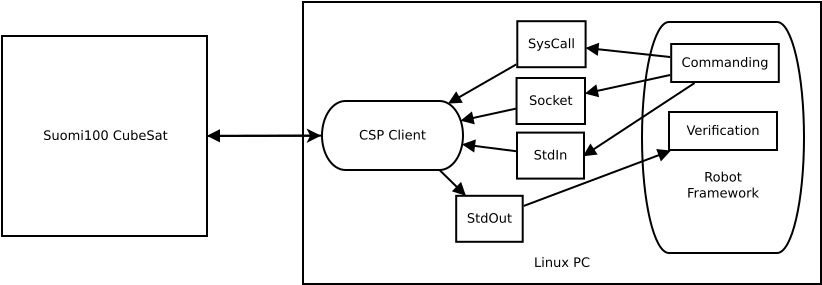
\includegraphics[scale=0.5]{cspautomation}
\caption{Illustration of the software architecture developed for Suomi100 test automation. Large rectangles represent environments, small ones represent layers and rounded rectangles represent programs.}
\label{cspauto}
\end{figure} 
\subsubsection{Python libraries}
A set of scripts using Python programming language were written, called
libraries in the context of Robot Framework. All of these libraries consisted of one Python class each. The class of the core library, known as \textit{CubeSatAutomation}, has the methods for the communication with the CSP client via any of the three methods, socket, Stdin or automated keypressing via pyautogui library. Furthermore the library includes the methods to read and verify the process replies from Stdout.
As can be seen in Figure \ref{cspauto}, the commands are sent to CSP client through any of the three communication routes and the output of the program goes to the Stdout. The output is then caught and read by the CubeSatAutomation library and test cases and test steps or keywords are failed or passed based on the output read from the CSP client. \par
It is importation to note the following details about the test automation libraries. 
\\
\\
\textbf{CubeSatAutomation library}\par
CubeSatAutomation library has the core functions for sending commands, opening socket connection, opening and closing the opened program and others. Besides being able to open the CSP client program, any program can be automatically opened with the library as the method for opening uses the standard Python \textit{subprocess} library. All the other libraries implemented use the core methods in CubeSatAutomation, for example, to send commands to the CSP client to execute. These other libraries have subsystem specific functions for the test automation. To create only one open communication route between CSP client and Robot Framework and to only one handle on the CSP client program process, the core library defines these as class variables, which are then accessed by the subsystem libraries. In practice this means that we don't open several CSP client programs and several connection routes separately for each subsystem library included in the test suite. Instead, the program and the communication route is opened only once for each test suite. Another class variable which defines the scope of the instance of the class in the Robot Framework was defined as well. This was chosen to have a value corresponding to the suite level, as the widely used \textit{Selenium2Library} uses the same scope for its class instance in Robot Framework as well. By having the scope on the suite level, only one instance of the library class is declared per test suite, thus again having only one handle on the client software and having only one connection route open during the execution of a test suite.\par 
The essential core methods used in the CubeSatAutomation Python class are explained below:\\
%\textbf{client_start(self, config_file=None, prog=None, params=None)}
\textit{\textbf{Client Start  <config file> <program> <parameters}}\\
Explain.\\
\textit{\textbf{Client Close <socket> <program>}}\\
Explain.\\
\textit{\textbf{Connect Socket <config file> <server> <port>}}\\
Explain.\\
\textit{\textbf{Send Command  <message> <option> <timeout> <read timeout>}}\\
Explain.\\
\textit{\textbf{Write Command  <message> <option> <timeout> <read timeout>}}\\
Explain.\\
\textit{\textbf{Type Command  <message> <option> <timeout> <read timeout>}}\\
Explain.\\
\textit{\textbf{Persistent Command  <message> <exception replies> <end reply> <timeout> <read timeout>}}\\
Explain.\\
\textit{\textbf{Verify Reply Contains  <message> <timeout> <read timeout>}}\\
Explain.\\
\textit{\textbf{Verify Reply Contains Not  <message> <timeout> <read timeout>}}\\
Explain.\\
\textit{\textbf{Verify Reply Contained  <message> <timeout> <read timeout>}}\\
Explain.\\
\textit{\textbf{Wait Until Reply Contains  <message> <timeout> <read timeout>}}\\
Explain.\\
Finally, here are some of the keywords presented that are specific to GomSpace NanoEye.\\
\textit{\textbf{Set Satellite Parameter  <device> <parameter> <value>}}\\
Explain.\\
\textit{\textbf{Send Satellite Parameters}}\\
Explain.\\
Remember to mention that replies can be stored temporarily.\par
Creation of a skeleton core library was the aim of the final development of our test automation library. This library only has the aforementioned methods to start and communicate with a desired Linux program running on terminal shell (or bash shell) and keywords that are more specific to Suomi100 or CSP client were omitted. With the aid of this library, satellite software developers wishing to automate testing of their satellite and satellite software, can then create their own specific libraries suited to their own needs. The final version of the CubeSat test automation library is desribed in section 4.\\
\\
\textbf{Subsystem libraries}\par 
Other libraries developed for test automation of Suomi100 are called \textit{NanoCam.py} and \textit{RadioPayload.py} and these were intended for the automated testing of NanoCam and radio payload subsystems respectively. The classes of both of these create an instance of CubeSatAutomation class instead of calling for specific functions or methods of that class. By doing this the class variables including handle to the automated process, socket address and others are passed to all these other classes as well. The methods of these classes thus use the methods of CubeSatAutomation directly.\par
The specific methods defined by the NanoCam test automation library are presented below as Robot Framework keywords:\\
\textit{\textbf{Camera Startup	<timeout>}}\\
Reboots the camera and downloads parameter table 1 from the subsystem. Timeout specifies the time that we wait for the camera subsystem to come online in satellite bus.\\
\textit{\textbf{Camera Take Picture	<timeout> <store format> <filename> <autogain>}}\\
Sets image format and filename in the camera and takes a picture with the given autogain value (empty at default). Keyword fails if the image is too dark (less 5 \% light) or too bright (over 95 \% light).\\
\textit{\textbf{Camera Load Picture	<stored file> <loaded file>}}\\
Downloads the file stored in NanoCam to the PC running CSP client program.\\
\par
The subsystem specific keywords for the radio payload are defined as the following:\\
\textit{\textbf{Radio Startup  <switch input> <switch power> <antenna input>}}\\
Explain.\\
\textit{\textbf{Radio Powerdown}}\\
Explain.\\
\textit{\textbf{Verify Radio Status}}\\
Explain.\\
\textit{\textbf{Run Radio Mode  <parameter file> <property file> <mode> <mode arguments}}\\
Explain.\\
\textit{\textbf{Verify Radio Results  <buffer file> <timeout>}}\\
Explain.\\
\textit{\textbf{Radio Load Data  <stored file> <loaded file> <timeout>}}\\
Explain.\\
\textit{\textbf{Radio Plot Data  <file> <output file> <plot image>}}\\
Explain.\\
  
 
\begin{itemize}
\item[--]Libraries are Static API version 
%http://robotframework.org/robotframework/latest/RobotFrameworkUserGuide.html#creating-test-libraries 
\end{itemize}     
\subsubsection{Robot framework test suites}
The test cases follow the keyword-driven approach and the keywords are written to be short and mostly to be non-specific to the test case. The functions and methods written in Python and described in previous section are used directly as such. Because the approach was to make smaller set of versatile and generic keywords that could be used over many test cases and test suites. This approach was felt to be more efficient as there would be less need to maintain the test suites if they had large set of specific, though descriptive, keywords. Besides, our satellite project is not a typical software project where stakeholders would go over the test suites and validate them. All people involved in the project have a technical background. In addition, having a set of general keywords that are not entirely tied to our satellite project is beneficial if some future satellite project wishes to use the testing methods and tools described in this thesis.\par
Each of the test cases are tied to a particular operation mode. The operation modes are discussed in detail in section 2.5. Purpose of each test case is to verify functionality of some aspect of the particular operation mode. Each test case is marked with the Robot Framework \textit{[Tags]} marker to identify which operation mode the test case is related to. The test suites are divided firstly based on the four different larger features what we are testing. Namely, separate sets of test suites are written for camera payload, radio payload, NanoEye basic functionality and for "Day in the life" testing. Each aspect of a feature further divides the test suites into test suites testing different parts of the particular feature.\par   
\subsection{Test setups and environment simulation}
As defined in section 2.5, different aggregates for testing were identified from Suomi100 satellite and for simulating the functional environment of the satellite for these different types of tests, four different environments were set up. Two different environments for testing two different payloads, one for testing basic operational features of the NanoEye platform and one larger for the operational scenario testing of the satellite. 
\subsubsection{Environment and setup for camera payload testing}
For the testing of the NanoCam and imaging operation mode, we tried to find something facing the camera with equal colour and brightness values as what the camera would see while in orbit. The easiest solution is to simply take the whole integrated satellite outside on a bright day to the balcony on top of our department in Aalto University. The satellite is standing on top of a stand and the side with the camera lense is directed towards horizon. A PC with CSP client and the test automation tools are connected to the satellite via the USB connection on NanoUtil. In addition, the satellite is loosely enclosed in a plastic container to protect it from particles in the air.\par 
Below is Figure \ref{camerabalcony} of the test setup used during the testing.\par 
\begin{figure}[h!]
\centering
\includegraphics[scale=0.3]{camerabucketspurgu}
\caption{Suomi100 satellite on a balcony during imaging mode tests.}
\label{camerabalcony}
\end{figure} 
\subsubsection{Environment and setup for radio payload testing}
Environment for the testing of the radio payload is set up in the clean room of Aalto University's space laboratory. The satellite is connected via the USB connection to a PC with the CSP client software and the test automation tools. The functional environment was simulated with a radio signal source in order to create some artificial noise in radio frequencies that would mimic the radio signals present in the ionosphere. The radio noise is generated with a \textit{HackRF One} Software Defined Radio (SDR) which is connected to another PC running \textit{GNURadio} signal processing software.\par 
Figure \ref{s100hackrf} shows the setup for the testing of the radio payload.\par   
\begin{figure}[h!]
\centering
\includegraphics[scale=0.3]{payload_testing_hackrf}
\caption{Radio payload testing with \textit{HackRF One}.}
\label{s100hackrf}
\end{figure}
The frequencies that are used in the environment simulation are 2 MHz, 5 MHz and 9 MHz. These were chosen based on the requirements of the payload (should operate in range of 1-10 MHz) and the limitations of the hardware, as the HackRF can't produce signals with lower frequencies than 2 MHz. Furthermore, the antennas attached to the payload themselves cannot receive signals that are much higher than 9 MHz. The middle frequency was chosen to be 5 MHz as based on the research done on the radio signals in the ionosphere, this frequency would be of most interest to us \cite{esanpapru}.\par 
Figure \ref{gnuradio} shows \textit{Fast Fourier Transform} (FFT) plot of the noise that is generated from the GNURadio, which is then transformed into radio waves by the HackRF.\par
\begin{figure}[h!]
\centering
\includegraphics[scale=0.45]{Test_window}
\caption{Screenshot from \textit{GNURadio} signal processing software showing FFT plot of a radio noise being generated.}
\label{gnuradio}
\end{figure}  
\subsubsection{Environment and setup for satellite basic operations testing}
For testing of the basic satellite operational features like collection of housekeeping and safe rebooting during an error, no external inputs to the satellite are used. The satellite is in the clean room of Aalto University's space laboratory connected to a PC with the CSP client. 
In Figure \ref{basictest} we have a picture of this setup.
\begin{figure}[h!]
\centering
\includegraphics[scale=0.3]{basicsetup}
\caption{Setup for testing of basic functionalities of the NanoEye platform. Suomi100 is on the left and a PC with CSP client and test automation softwares is on the right.}
\label{basictest}
\end{figure}  
\subsubsection{Environment and setup for satellite operational scenario testing}
In "day in the life" operational tests, the Sun is simulated with a %\textit{Philips BMH 1800L 55} 
1800 Watt Xenon lamp that is situationed approximately 1.5 meters away from the satellite. Two solar panels are connected to the satellite in the manner they are connected during flight. The satellite faces the lamp in an angle so that both panels receive light from the lamp. As the lamp is quite powerful, we can really verify that the solar panels charge the batteries in the satellite. In addition, the lamp can heat the objects it is faced towards and this was used as a method to add some thermal features to the test. The idea is to use the lamp for the time it takes the satellite to heat up to 50 degrees celcius under the illumination and to then let it cool back to room temperature (approx. 27 in our clean room). The heating and cooling was measured with \textit{FLIR E6} thermal camera and the heating time was measured to be approximately 10 minutes and the cooling down period was measured to last ca. 20 minutes.\par
In Figure \ref{dayinlife1} this setup with the solar simulator is presented.\par
\begin{figure}[h!]
\centering
\includegraphics[scale=0.3]{daysetuplamp2}
\caption{Day in the life setup for the satellite. The Xenon lamp is on the left and Suomi100 CubeSat is on the right in the picture.}
\label{dayinlife1}
\end{figure} 
For the "day in the life" testing, these periods form the phases of the operational scenarios. When we pretend that the satellite comes from eclipse, we turn on the Xenon lamp and we are in communication with the satellite for 10 minutes and after that the lamp is turned off and we pretend that the satellite goes out of the reach of our ground stations and stays there for 20 minutes. In addition, the 10 minutes communication window roughly corresponds to the time that we can be in communication with the satellite during one revolution around Earth by the satellite.\par 
Unlike in the setups described previously, the control of the satellite happens via radio link. A SDR with model \textit{Ettus USRP B200} is connected to a PC with the CSP client software and the test automation softwares. This SDR is the one used in the actual ground station and for this testing the SDR and the PC were located in the next room in Aalto University's space laboratory. The actual groundstation and all of its hardware is not used because the solar simulator has to be controlled manually and the groundstation is situated several floors up from the Aalto University's Space laboratory.\par 
Figure \ref{dayinlifelink} presents this setup.\par
\begin{figure}[h!]
\centering
\includegraphics[scale=0.3]{daysetuplink}
\caption{Day in the life setup for a "stripped down" groundstation.}
\label{dayinlifelink}
\end{figure} 
\clearpage
\section{Results and Discussion}
%\section{Tulokset}
\subsection{Executed tests}
The Robot Framework test suites executed can be divided into three categories: test suites done for the two payloads (1), test suites written for general satellite operations (2) and test suites for "day in the life of the satellite" operational scenario tests (3). \par 
The first category of suites follow more traditional method of combinatioral testing. Each test case was derived from the operation modes defined for the camera and radio payloads. Each of the test cases for their representative operation mode are identical in steps, but use different combination of values in the keyword arguments. \par
The second category consists of test suites made for the functional testing of the commands that contribute to the basic operations of the satellite. These test cases for different operations are completely different from each other and the tests here begin to resemble different scenarios or use cases. Such as telemetry gathering, flight planner commands, software update, etc. In addition, test suite was written for testing restarts of the subsystems and of the OBC and of the whole satellite as well.\par 
The third category, follows the higher level satellite integration tests where we test the satellite based on operational scenarios. Separate test suites were written for each operational scenario. The test cases at this level are simply different phases in the operational scenario.\par
In addition to these test suites, another one was used during the development of the software for the radio payload. This test suite resembles a smoke test and it has limited set of test cases, testing each of the operation modes. Yet, no proper continous integration chain was done during this time, but the smoke tests were manually started usually once every week.\par   
\subsubsection{Tests for camera payload}
The test cases for the NanoCam were identical in structure, or in other words, we made several test cases for the same use case of the camera payload. Only difference was that the main parameters like gain value and exposure time differed between test cases. These two are the main parameters according to the NanoCam manual provided GomSpace \cite{nanocamds}. Having the exposure time fixed, we demonstrated the use of combinatorial testing to go through different variations of the camera parameters. Three different values of the exposure time were used and for each value, the same parameters other than exposure time were changed in different test cases. The values used for the exposure time were ${10 ms}$, ${30 ms}$ and ${90 ms}$.  Below is Figure \ref{robotcamera} showing the test case structure used in testing of the camera payload.\par
\begin{figure}[h!]
\centering
\includegraphics[scale=0.5]{cameracase}
\caption{Robot Framework test case structure for camera payload testing. The 1st column represents the command or action performed in CSP client (see section 3.2.2-3.3.3), second, third and fourth columns define parameter options and values for the commands.}
\label{robotcamera}
\end{figure}
As can be seen from the example test case, the test covers such features as NanoCam restart and detection in the satellite bus, the use of different camera parameters and finally, image taking, storing and transfer from the satellite. All taken images were then added to the Robot Framework log files, which gives a comprehensive view on how the different camera parameter values affected the taken images.\par 
For the environment simulation, the attempt was to find a really sunny day to give some indication of the brightness of the pictures while the satellite is in orbit. This was achieved to some extent, but at the start of the test few clouds appeared and some pictures turned out very bright and some less so. If the level of light would have stayed the same during the whole test, we could have gotten some baseline information about the affects of the different parameters on the images.\par
Nonetheless, no test cases failed due to software errors. These tests on the camera provided certain confidence that changing different parameters didn't crash the software or that any combination of parameters didn't cause problems in the functioning of the satellite. We also observed that the images didn't become distorted in any way. Out of the 39 test cases, 9 failed because the light level was too high. Yet, the brightness in space around Earth is much higher than what we can have here on the surface even at the brightest day [source], not to mention the fact that the tests were conducted in Finland. Thus, increasing the exposure time or gain value while in orbit will make the images to be too bright and therefore, setting the camera parameters to their default values would possibly give us the best pictures. One should recall that, the automation of these tests was the first time our automation libraries along with Robot Framework were used to properly test Suomi100 satellite and therefore these tests worked as a technology demonstration as well. Figures \ref{camerapic1} and \ref{camerapic2} show some pictures taken with the NanoCam camera on the Suomi100 satellite. \par
Most importantly, the tests demonstrated that the integration with the rest of the satellite was succesful. As in fact, there was a defect in the integration of the camera with the satellite at the first time the satellite platform arrived to us. The camera lense was too far away from the cell in the PCB of the camera subsystem and the first test pictures taken with the camera were distorted. The manufacturer of the satellite platform provided us with a test picture that the camera was working properly, but it seems that they didn't test the camera after it was integrated to the satellite. After this problem was found, GomSpace provided us with a new camera and the integration of this worked properly. The Robot Framework tests worked thus also as the verification tests for the integration of the NanoCam subsystem to the satellite platform.\par 
\begin{figure}[h!]
\centering
\includegraphics[scale=0.2]{def}
\caption{Picture taken at Maarintie 8, Espoo, with NanoCam integrated on the Suomi100 satellite. Camera parameters were set to the default values provided by NanoCam manual \cite{nanocamds}.}
\label{camerapic1}
\end{figure}
\begin{figure}[h!]
\centering
\includegraphics[scale=0.2]{def23}
\caption{Picture taken at Maarintie 8, Espoo, with NanoCam integrated on the Suomi100 satellite. Camera parameters were set to use exposure time of 30 milliseconds and to use no gamma correction.}
\label{camerapic2}
\end{figure}
\subsubsection{Tests for radio payload}
During the development of the software for the payload radio, a small test suite was used for smoke testing of the software and the payload. Basically, the test cases tested that the general commands are executed without errors and that the radio can output data. This test suite was also used when the payload was integrated to the satellite.\par
The three tests in this suite were run at least once a week during the development of the software, but a proper \textit{Continuous Integration/Continuous Development} (CI/CD) pipeline was not used where for example flashing of a new software to the NanoMind would have caused these test to run automatically.\par
Besides the aforementioned smoke test, a more comprehensive set of test suites was performed for the radio payload after it was confidently integrated to the satellite platform. As the hardware and software were of our own design and the system integration occurred with a platform manufactured by another organization, these tests took the most time of all automated tests done on Suomi100 satellite. A few sessions were held where we ran these comprehensive test suites for the radio payload and each time new defects in the code and in the integration were found. Of all the tasks related to Suomi100, the proper integration of the radio payload to the GomSpace 1U NanoEye took the most effort from us.\par
Test cases for our payload followed the combinatorial testing method in a way where all the the test suites for a given radio operation mode had the same test cases but the frequency used was different. In addition, the test suites for different radio operation modes differed as each had a bit different parameters. These test suites then covered some amount of different parameter combinations and as with the camera payload, the measurement data was downloaded from the satellite and then processed and plotted and the figures were added to the Robot Framework HTML log files.\par 
In Figure \ref{robotradio} is an example of the test case structure used in testing of the radio payload.\par 
\begin{figure}[h!]
\centering
\includegraphics[scale=0.5]{payloadrfwtest}
\caption{Robot Framework test case structure for radio payload testing.}
\label{robotradio}
\end{figure}
Most interesting information about the payload operation was found from the CSP client replies outputted to the log files. What we were measuring was static and as such, nothing too much could have been said about the test cases just by looking the measurement plots. Besides the fact that the values were not zero or that there was actual variance in the values measured. In Figure \ref{m1_debug1joo} below we have one plot produced from measurement made with the radio while the satellite was at our laboratory at Aalto University and no external radio signal sources were generated by us.\par 
\begin{figure}[h!]
\centering
\includegraphics[scale=0.6]{m1_debug1}
\caption{Plot of measurements of radio static made by the radio payload at 5 MHz.}
\label{m1_debug1joo}
\end{figure}
During integration and testing of the radio payload, several problems occurred. Some of these problems can be attributed to be \textit{emergent problems in integration}. For one, the payload was developed so that a \textit{RaspberryPi 3} computer simulated the OBC. This computer has a Quad Core 1.2 GHz processor from Broadcom [source] and the processor in the NanoMind OBC in Suomi100 is a 32 MHz processor with a single core \cite{nanomindds}. While the data from the payload can be read and stored within the 31.25 microseconds with the RaspberryPi 3 to have a sample rate of 32 kHz at lowest, the reading and storing with NanoMind takes considerably longer, over 60 microseconds. In addition, we need to read the data two times before obtaining a completely new measurement value. This because the payload outputs the data from two audio channels, left and right, and we are reading the data from one channel at a time. Therefore, with the NanoMind OBC, we can theoretically have a sample rate of 8 MHz.\par
In addition, it was found that the reading and storing even at this rate is not consistent as the FreeRTOS runs other tasks while we are reading data from the payload. Figure \ref{payloadosc1} shows a screenshot from a \textit{Tektronix TBS 1072B-EDU} oscilloscope reading the \textit{slave select} pin from the payload. When the value of the slave select is low, a single reading of data from the instrument has happened.
\begin{figure}[h!]
\centering
\includegraphics[scale=0.5]{F0001TEK}
\caption{Screenshot from a Tektronix oscilloscope showing inconsistency in data reading rate from the radio payload instrument.}
\label{payloadosc1}
\end{figure}
In an attempt to counter this, we first increased the priority of the FreeRTOS task assiocated with the operations of the radio instrument to highest among all the tasks in NanoMind. This didn't improve the situation though. Thus, we made our task to call for a FreeRTOS \textit{vTaskSuspendAll()} command, which would give all the processing power of the processor for our task and freeze all the other tasks in the OBC. This caused some \textit{watchdog} process unknown to us to reboot the computer, which possibly assumed that the computer was "frozen" and as a safety feature rebooted the computer.\par
Therefore, as a compromise the sample rate was dropped down to 1 kHz. This was done by adding a \textit{vTaskDelay(1)} command to our FreeRTOS task after every read and store cycle. This was the shortest time we could add to our task, a shorter wait time would have possibly given a higher sample rate. But, this would have required us to modify the general definitions of the NanoMind code, which could have caused unforeseen consequences to the operation of the satellite. Figure \ref{payloadosc2} shows that on certain periods we can obtain the data more consistently. Yet, during a longer time period, there still exists longer gaps between data reading events than what we could anticipate. Nonetheless, this data rate seems to be good enough for our needs. Though, any "real-time" radio noise that could be listened from the radio instrument by human ears is not feasible with this setup.\par
\begin{figure}[h!]
\centering
\includegraphics[scale=0.5]{F0003TEK}
\caption{Screenshot from the oscilloscope showing better consistency with lower sample rate in data reading rate from the radio payload instrument.}
\label{payloadosc2}
\end{figure}
In addition to the data rate problem, some problems were discovered with the payload and the Nanomind themselves. For the command to tune the frequency in the si4740 IC, an automatic antenna capacitance calculation was supposed to happen for a given frequency. Yet, from the Robot Framework log files it was found that the antenna capacitance value was always $1$. Thus, we had write a separate command ourselves which calculates the capacitance value. In the consequent tests with this modification, the values seemed to be correct and it could also be seen from the figures plotted from the measurement data.\par 
Another issue which was faced involved the GPIO pins in the NanoMind. We would have required four of them for our needs, yet only three out of six worked for us. By changing the purpose of these three pins in relation to our payload instrument was sufficient. This made it possible for us to read the data in the first place.\par 
As a conlusion to the radio payload, the subsystem would have required its own processor and its own flash memory in order to have higher sample rate and with more consistent data reading and storing. As is the case with the NanoCam subsystem, which has a 536 MHz processor and 2 Gigabytes of non-volatile memory for image storage. Nonetheless, even with a very low sample rate, we can gather some valuable information from the ionosphere [sources?].    
\subsubsection{Tests for basic satellite operations}
Testing of the basic functionalities of the satellite software is necessary in order to obtain a reliable satellite. Therefore, tests were performed for satellite features such as safe satellite reboots, different housekeeping commands, flight planner commands and flight software updating. All of these can be seen as the basic functionalities which all of the other operations of the satellite depend upon. Test suites for these features don't follow the combinatorial testing methods used for two payload subsystems. Instead, test cases are based on different use cases or different situations we might end up facing with the satellite. In addition, the keywords used were less subsystem specific and more of the test cases used the generic keywords, such as \textit{Send Command} and \textit{Verify Reply Contained}.\par
\textbf{Reboot tests}
\par 
Twelve test cases were written for satellite reboots during different situations. The goal of these tests was to find out if during some operation, e.g. file upload, we can get the NanoMind "frozen" so that it doesn't reboot safely anymore. This test suite also has test cases simply to shutdown different subsystems and to verify their absence in the satellite bus with the simple \textit{ping} command. From these test cases, it was found that the NanoCom communication system couldn't be shutdown completely. It still replied to ping commands even though a command was sent to shut it down. This functionality naturally is preferable (NanoCom manuaali sanoo tästä jotain?) and though this led to one test case of the reboot test suite to fail, the test can be seen to fail positively. As such, eleven test cases passed and one failed positively from this test suite. \par
The other types of test cases in the reboot test suite tested reboots during satellite operations and the reboots were mostly caused by adding reboot commands to the flight planner so that they would occur during some satellite operation, e.g. during radio payload operation. In all of these, the satellite came back safely. Yet, it has been several times that the NanoMind can get stuck and in those situations to get the OBC working again, it has required us to either manually reboot the EPS or to send a command via another subsystem to reboot the NanoMind. The satellite has recovered safely from these situations after reboot. But when we are using the satellite control software, CSP client, we are not able to do this. This situation arose the question whether there can happen something during orbit that causes the satellite to be "frozen" forever.\par
Fortunately, there are several watchdogs in the satellite that in theory can trigger a reboot after a certain time. Unfortunately, we were not able to deliberately trigger a situation where NanoMind is stuck and thus tests for these watchdog functionalities had to be omitted from the test suite.\par 
\textbf{Housekeeping tests}
\par 
Another eleven test cases were performed to test the housekeeping features provided by the GomSpace platform. Test cases were written for different housekeeping commands of different subsystems as well as for housekeeping data storing and transfer from the satellite. Testing of the beacon functionality was as well included in this test suite, as the beacon outputs recent HK information. Plotting of the beacon data was developed during the realization of these tests by another member of the satellite team, M.Sc Petri Koskimaa, and by the thesis author. These plotting functionalities were later used in the "day in the life of the satellite"-tests as well. All test cases of this test suite passed without errors. This means that, all the commands did what they were supposed to do, which was obviously the preferred result. In Figure N we have an example picture of a plot of the system current provided by the beacon at different timestamps.\par 
\begin{figure}[h!]
\centering
\includegraphics[scale=0.6]{hk_plot_cam_op2}
\caption{System current from the beacon data during imaging mode operation mode.}
\end{figure}
\textbf{Flight planner tests}
\par 
For testing of the flight planner feature, seven test cases were performed. The feature was tested with some basic flight planner creation commands as well as with more complicated ones. Out of all these tests involving basic functionalities of our satellite, this one had the most failed test cases. For first, it was assumed that giving the commands in wrong format (string instead of an integer) would cause the CSP client to indicate an error. Such a thing didn't happen but giving the commands in wrong format didn't cause the software to crash either. In addition, if the command string was too long, an error was indicated and no flight planner command was appended to flight plan list. Which happened to be the case when we tried to give one specific command for our radio payload, but this command to run the radio payload in one of the defined operation modes happens to be the single most essential command for the payload. Therefore, in order to make it work with the flight planner we need to modify the source code for the flight planner so that it can accept longer strings as commands (ei tehty vielä!). Otherwise, we can only use the radio payload when the satellite is in the reach of our communication radios. This is not preferrable as we would be radically limiting the area what we can measure.\par
\textbf{Software update tests}
\par 
Three test cases were performed for the software update feature. These test cases took a longer time to run than the other test cases involving the basic functionalities of the satellite, because we had to upload the new software to the satellite via the USB on the NanoUtil. These tests tested basic uploading of a new software image, rebooting back to the software that was flashed to NanoMind and tested uploading of an invalid file as an image to the new software. The satellite passed all these tests as expected giving us some confirmation that we actually can upload a new software to the satellite and command it to reboot with that software.\par
In the test case where we uploaded and invalid file as an image, the file itself was just a binary file containing measurement values from the payload radio. Booting with this file caused the NanoMind to crash with EXCEPTION 13 error message. In addition, we had set the NanoMind to try to boot with this file three times and it crashed each time with this error. Eventually as the boot counter reached zero, the satellite managed to recover the proper software it was flashed with. This test gave us knowledge that the satellite manages to recover itself if we happen to upload a software to the satellite that causes unexpected reboots.\par
\subsubsection{Tests for "day in the life" operational scenarios of the satellite}
Test suites were formed to test different phases of the scenarios that the satellite will encounter while in orbit. A scenario would be e.g. where we come from the eclipse, send commands to the satellite and downlink data. Each step in the scenario, like downlinking of data, formed its own test case within the test suite. 
Four different operational scenarios were tested. These are described as:
\\
\par 
\textit{1: The satellite comes from eclipse and is in the reach to form a radio link with the groundstation. Housekeeping data is gathered, the satellite takes an image and a measurement is made with the radio payload. Afterwards, the housekeeping data and the measurement are downloaded from the satellite. Finally, the satellite goes out of the reach of the groudstation.}
\\
\par 
\textit{2: The satellite comes from eclipse and is in the reach to form a radio link with the groundstation. Housekeeping data is gathered and flight planner is used to set the camera to take a picture while the satellite is in eclipse and out of the reach of the groundstation. After the satellite has orbited the Earth, the satellite comes again from the eclipse and is in the reach of the groundstation. Housekeeping data and the taken image is downloaded from the satellite. The satellite goes again out from the sight of the groundstation.}
\\
\par 
\textit{3: The satellite comes from eclipse and is in the reach to form a radio link with the groundstation. Housekeeping data is gathered and flight planner is used to set the camera to take pictures continuosly. Flight planner is used to gather housekeeping data continuosly as well. A reboot happens presence of all subsystems is verfified. The camera is given a command to take a picture to verify the basic operation of the subsystem. In addition, verification for the charging of the batteries via the solar panels is verified. Finally, the housekeeping data is downloaded from the satellite.}
\\
\par 
\textit{4: The satellite comes from eclipse and is in the reach to form a radio link with the groundstation. Housekeeping data is gathered and flight planner is used to set the camera to take pictures continuosly. A file is uploaded to the satellite and finally the satellite goes out of sight of the groundstation.}\\
\\
One test suite for each scenario was written. Different phases of a scenario were made in to different test cases in the suite. Majority of the keywords used in the test suites were the \textit{Persistent Command} and \textit{Verify Reply Contained} keywords. Persistent commanding was required for majority of the commands because the radio link was not entirely stable. The test suites were executed several times and occasionally some keywords caused the test cases to fail due to the connection being temporarily lost.\par
Control of the solar simulator was not automated due it being just a lamp that one attaches to the electric plug to turn it on. Thus in practice the person responsible for the testing had to manually plug and unplug the simulator from the mains current. Therefore, another keywords were written for these tests which with a sound effect indicated that the lamp had to be turned or to be turned off. These were the \textit{Wait And Notify}, \textit{Notify After}, \textit{Wait Until Time event} keywords.\par
One of the important aspect with these tests was verification that the solar panels charge the batteries. All the test suites had at least one test case for battery charging verification. In all such cases, the solar panels were detected and they did infact charge the batteries. As presented in section 2.1, one of the potential causes for failures with previous CubSats has been that the solar panels were not properly connected to the power bus \cite{Swart1}. Thus, testing of this was felt to be necessary. Figure \ref{epsvbatt} shows how the charge in the batteries changed over the execution of the first scenario.
\begin{figure}[h!]
\centering
\includegraphics[scale=0.6]{hk_plot1}
\caption{EPS battery charge from the beacon data during first defined satellite operational scenario.}
\label{epsvbatt}
\end{figure}  
All the test cases for scenario 1 were executed succesfully. The housekeeping data and radio measurement were downloaded from the satellite succesfully via the radio link. Similarily, all test cases for scenario 3 succeeded. A reboot was caused in the satellite and all the subsystems responded to \textit{ping} commands after the reboot. We were able to again take an image and verify that the solar panels were again charging the satellite. Test cases for scenario 4 were passed as well and a file was uploaded succesfully to the satellite.\par 
Some problems emerged with testing of scenario 2. Namely, the download speed was too slow to enable us to download an image from the satellite during the time defined for the scenario. As presented in section 3.3.4, the time that the satellite is in the sight of the groundstation is approximately 10 minutes. The image taken by the camera was roughly 300 kilobytes in size and during the time we downloaded it, we received roughly 53 kilobytes.\par 
One reason for the slow download speed was the setting for \textit{rdpopt} command, which defines the wait times between each packets received among other things. With a short wait time the time between received packets is shorter, but the connection during downloading can be lost more frequently. With a longer wait time, the speed is lower but the connection is more stable. The theoretical maximum speed for downloading in our case is $0.9 kb/s$. From the test suite logs we could see that at best we could receive data at the speed of $0.3 kb/s$. Therefore, some fine tuning of the \textit{rdpopt} command parameters would be needed to practically make the download faster.\par
As a conclusion, it was verified that the solar panels did charge the batteries and the communication with the satellite over the radio link worked. All the commands sent to the satellite worked as they were supposed to. Only the download speed was too slow so that we couldn't download a full picture from the satellite. Besides this, all the test cases passed.\par      
\subsection{Release version of CubeSatAutomation test library}
The release version of the core function library, \textit{CubeSatAutomation}, was cleared from Suomi100 related dependencies and only the generic process communication keywords are present. Explain some strategy in process communication (only some \textit{Run Command} and \textit{Run Command Persistently} keywords are used and the software knows how to choose between, send, write and type.)\par 
Automation of several Linux terminal programs were tested with the test library succesfully. It was decided that library would be available for everyone who wishes to use test automation with terminal based programs (like some groundstation softwares), thus the library can be found in GitHub. In addition, some example Robot Framework test suites using the CubeSatAutomation library were added to the repository. Any team willing to use the library for test automation with Robot Framework would easily be able to start automating their groundstation software.\par  
%pip install -r requirements.txt  
%pip install -e . (setup.py tarvitaan) 
\subsection{Developing operational scenario tests as requirement for CubeSat mission readiness: "Day in the Life of a CubeSat"}
Lue "improving mission success..". Conclusion, at minimum, day in the life, communication with groundstation, power system charge/discharge, thermat testing in vacuum. Day in the life, samoja mitä tehtiinkin.\par
Currently the CubeSat standard demands the following tests to be performed for a satellite: \textit{Random Vibration}, \textit{Thermal Vacuum Bakeout}, \textit{Shock Testing} and \textit{Visual Inspection} \cite{cds}. These are demanded only for the reason of ensuring safe integration of the P-POD deployer and the CubeSat in to the launch vehicle. The specifications for these tests in fact usually are defined by the launch provider \cite{cds}.\par 
As can be seen, no testing is required for electrical or functional/operational testing of the satellite. In the research data represented in section 2.1 it was found that failure rates from 40 \% to 20 \% were prevalent in CubeSat missions \cite{Swart1, Swart2016, Swart2015}. In addition, it was suggested that these high failure rates were attributed to poor or nonexistent functional system integration testing. More so, understanding of integration and testing could have been something lacking from the University led CubeSat teams. In comparison, the CubeSat missions that were led by organisations and companies with vast experience in satellite integration and testing had considerably lower failure rates.\par 
Therefore, we are suggesting at least for some form of guidelines for functional integration testing to be added to the CubeSat standard. Study for creation of such guidelines is deemed to be necessary. These guidelines could be devised from the experiences of previous succesful CubeSat missions as well as from the experiences and used testing practices of the "traditional" space missions.\par
In section 2.5, the represented research on failures with larger spacrafts also pointed to the lack of proper integration and testing as a source for mission failures. In addition, when the established testing practices used in NASA were "streamlined", consequent missions showed significant decrease in performance. When comparing the data from failed CubeSat and traditional space missions, it could further be claimed that at least some guidelines for integration testing are needed for the CubeSat standard. \par
In addition, a "Day in the life" operational scenario tests are required for NASA and ESA missions \cite{tor}. Besides the mechanical tests mentioned, a test following that principle could be devised for another test that is required from CubeSats. A test known as \textbf{\textit{"Day in the life of a CubeSat}}. Test like this would test the functionality and proper integration of the satellite. The communication with the groundstation could likewise be verified. The scenarios that would be tested could possibly be planned according to the guidelines given for functional testing of CubeSat. In theory, this test could decrease the amount of DOA cases for CubeSat missions. As noted in \cite{Swart1, Langer} one of the alleged reasons for CubeSat failures has been improper integration of the solar panels to the satellite and thus not having enough power to form the radio link with the groundstation. A test like the one discussed here could on ground verify these two aspects of the mission.\par
One technical solution for a "Day in the life of a CubeSat" test is presented in this thesis. Which includes the integrated satellite, a solar simulator and the groundstation. Some basic scenarios for satellite operations were devised and tested. The mechanical stress tests for CubeSats are performed with automated machinery, likewise a method to automate "Day in the life of a CubeSat" is presented in this thesis. This test automation includes Robot Framework and the function libraries developed by us. The final version of the function library was made to be a generic testing library, which is able to automate the use of many programs running in terminal environment. Therefore, many other groundstation control softwares could possibly be automated, given that they are terminal based. A setup for a "Day in the life of a CubeSat" test is presented in Figure \ref{dayinlifediagram}.\par
\begin{figure}[h!]
\centering
\includegraphics[scale=0.6]{dayinlifesetupdiagram}
\caption{Presentative diagram for a "Day in the life of a CubeSat" test with automated control of groundstation and solar simulator.}
\label{dayinlifediagram}
\end{figure}   
Documentation for a "Day in the life of a CubeSat" is another aspect that should be considered. Perhaps, the rigorous methods used in NASA [source] could be avoided and a more subtle method could be devised. Starting from design for operational scenarios to features to be tested and finally to documentation of passed and failed test cases.\par
  
Similar to testing for mission readiness at this level done by NASA and others, but "simpler"?\par 
What kind of documentation? Is it affordable for all CubeSat teams?\par
% Test suites like the ones were written could be run continuosly over several days even. Thus we could truly make tests for the life of the satellite and automate the whole testing. "Real" satellites could also benefit from this.
\subsection{Further lessons learned from testing of Suomi100 CubeSat}
More rigorous requirement specifications, they would help higher level functional testing.
What it should do, what it shouldn't do. Some area of operation, etc. More rigorous identification of operational scenarios and operation modes. All these in the vein of the CubeSat concept, not too rigorous or too formal, yet covering all the situations. Some examples from industry or other CubeSat missions?\par  


%% Huomaa seuraavassa kappaleessa lainausmerkkien ulkopuolella piste, 
%% koska piste ei lopeta lainattua tekstinp\"atk\"a\"a.
%% Jos lainattu tekstinp\"atk\"a loppuu v\"alimerkkiin, tulee v\"alimerkki
%% lainausmerkkien sis\"alle: 
%% "Et tu, Brute?" sanoi Caesar kuollessaan.


\clearpage

\section{Conclusions} 
%\section{Yhteenveto}
In this thesis automated functional system integration tests for Suomi100 CubeSat were performed with Robot Framework. The need for testing at this level was identified from surveys conducted for all CubeSat missions flown previously, which showed a high failure rate for University led missions in contrast to low failure rates for missions performed by organisations and companies with established practices in integration and testing. Thus, testing methods used by e.g. NASA at satellite integration level along with industry proven testing practices were applied in design of testing performed for Suomi100. The testing was automated with Robot Framework, which is an industry proven acceptance testing framework. It was felt that doing the testing with the help of an automated computer software would give the testing more rigour and reproducibility. For automating the control of the satellite in interest of test automation, libraries for use with Robot Framework were programmed with Python programming language.\par
First tests conducted for the satellite were functional tests for integrated Suomi100 payloads, which are an optical camera and a radio instrument for ionospheric measurements. Second test set included acceptance testing of the core satellite functions  such as housekeeping data collection, safe reboot handling, software updates and so forth. Final set consisted of tests for operational mission scenarios or "day in the life of the satellite"-tests.\par 
An attempt was made with our limited resources to simulate the functional environment for testing of the payloads as well as for the operational scenario tests. For testing of the camera payload, the satellite was taken to a balcony at our department on a sunny day. During the testing of the integrated radio payload,  a HackRF software defined radio was used to simulate the noise signals found in the ionosphere. A larger setup was used for the "day in the life of the satellite"-tests. With this test, we tested not just the proper functionality of the satellite software but that the radio link to the satellite works and that the solar panels can charge the satellite. Thus, the automated tests were performed via the radio link and a large Xenon lamp was used to simulate the Sun.\par 
With the performed tests, we proved proper functionality of the camera payload as well as proper functionality for almost all of the tests conducted for the core satellite functions.   The operational scenario tests showed that we can communicate with and send commands to the satellite via radio link and that the solar panels can charge the batteries in Suomi100. Only downside seemed to be the low downlink speed, yet this was to be expected.\par 
The tests for the radio payload on the other hand presented several defects and most importantly emergent problems in the integration with the rest of the satellite platform. The defects were fixed with consequent software updates, but certain problems with integration couldn't be overcome. The biggest one being the slow speed of reading and storing of data from the payload by the OBC. This forced us to drop the sample rate from the possible 32-48 kHz to just 1 kHz for reliable data measurement.\par  
Performing of these tests proved to us that Robot Framework can work as a testing framework for CubeSats and that we could carry out automated testing of Suomi100 CubeSat. The software libraries doing the actual automation were developed into a generic testing library, which potentially could be used for testing and automation of any Linux terminal software, such as a satellite ground station control software.\par 

\begin{itemize}
\item[--]Did we improve the functionality and reliability of the satellite?
\end{itemize}



\clearpage
%% L\"ahdeluettelo
%%
%% \phantomsection varmistaa, ett\"a hyperref-paketti latoo hypertekstilinkit
%% oikein.
%%
%% The \phantomsection command is nessesary for hyperref to jump to the 
%% correct page, in other words it puts a hyper marker on the page.

\phantomsection
\addcontentsline{toc}{section}{\refname}
%\addcontentsline{toc}{section}{References}
\begin{thebibliography}{99}

%% Alla pilkun j\"alkeen on pakotettu oikea v\"ali \<v\"alily\"onti>-merkeill\"a.
\bibitem{aftersputnik} Collins, Martin
  \textit{After Sputnik: 50 Years of the Space Age}, Smithsonian Books, HarperCollins, New York, USA, 2007.
\bibitem{rocketeers} Belfore, Michael,
  \textit{Rocketeers: How a Visionary Band of Business Leaders, Engineers, and Pilots Is Boldly Privatizing Space}, \nth{1} edition, Smithsonian Books, HarperCollins, New York, USA, 2007.
\bibitem{Swart1} Swartwout, Michael,
  \textit{The First One Hundred CubeSats: A Statistical Look}, Journal of small satellites, 2013. 
\bibitem{pluto} 
  \textit{http://pluto.jhuapl.edu/}, obtained 8th of March 2018. 
\bibitem{satcommunications} Pratt, Timothy, Charles W. Bostian \& Jeremy E. Allnutt,
  \textit{Satellite Communications}, \nth{2} edition, John Wiley \& Sons, New Jersey, USA, 2003.
\bibitem{filaw} 
  \textit{https://tem.fi/en/spacelaw}, obtained 23rd of February 2018.
\bibitem{cds} The CubeSat Program,
  \textit{CubeSat Design Specification Rev. 13}, California Polytechnic State University, 2014.
\bibitem{iceye}
  \textit{http://markets.businessinsider.com/news/stocks/iceye-successfully-launches-world-s-first-sar-microsatellite-and-establishes-finland-s-first-commercial-satellite-operations-1012996541}, obtained 23rd of February 2018.
\bibitem{Swart2017kalvo} Swartwout, Michael
  \textit{CubeSats and Mission Success: 2017 Update (with a closer look at the effect of process management on outcome)}, NASA Electronic Parts and Packaging (NEPP) Program
2017 Electronics Technology Workshop, Maryland, USA, 26-29 June 2017.
\bibitem{nasacubesat1}
  \textit{https://www.nasa.gov/mission\_pages/station/research/benefits/cubesat}, obtained 23rd of February 2018.
\bibitem{spacesystemsengineering} Fortescue, Peter et al.,
  \textit{Spacecraft Systems Engineering}, \nth{4} edition, John Wiley \& Sons, USA, 2011.
\bibitem{openorbiter} Straub, Jeremy et al.,
  \textit{OpenOrbiter: A Low-Cost, Educational Prototype CubeSat Mission Architecture}, Machines 1:1-32, 2013.
\bibitem{reliabilitycubesatelbus} Bouwmeester Jasper et al,
  \textit{Survey on the implementation and reliability of CubeSat electrical bus interfaces}, CEAS Space J, 9:163-173, 2017.
\bibitem{sularikurssi} Laplante, Phillip A. \& Ovaska Seppo J.,
  \textit{Real-Time Systems Design and Analysis}, \nth{4} edition, IEEE Press, USA 2012.
\bibitem{artofsofttesting} Myers, Glenford J.,
  \textit{The Art of Software Testing}, \nth{3} edition, John Wiley \& Sons, New Jersey, USA, 2012.
\bibitem{testingcomplex} Pries, Kim H. \& Quigley Jon M.,
  \textit{Testing Complex and Embedded Systems}, Taylor and Francis group, CRC Press, USA 2011.
\bibitem{systinttesting1} Kandl, Susanne et al.,
  \textit{A Formal Approach to System Integration Testing}, European Dependable Computing Conference, United Kingdom, 2014.  
\bibitem{Swart2016} Swartwout, Michael,
  \textit{Secondary Spacecraft in 2016: Why Some Succeed (And Too Many Do Not)}, Saint Louis University , 2016 IEEE Aerospace Conference, Montana, USA,  5-12 March 2016.
\bibitem{csdatabase}
  \textit{https://sites.google.com/a/slu.edu/swartwout/home/cubesat-database}, obtained 19th of March 2018. 
\bibitem{SpaceWorks2017} Doncaster, Bill \& Williams Caleb \& Shulman Jordan,
  \textit{2017 Nano/Microsatellite Market Forecast}, SpaceWorks Enterprises, Inc. (SEI), Atlanta, USA, 2017.
\bibitem{Swart2015} Swartwout, Michael,
  \textit{Secondary Spacecraft in 2015: Analyzing Success and Failure}, Saint Louis University, 2015 IEEE Aerospace Conference, Montana, USA, 7-14 March 2015. 
\bibitem{Langer} Langer, Martin \& Bouwmeester Jasper,
  \textit{Reliability of CubeSats - Statistical Data, Developer's Beliefs and the Way Forward}, \nth{30} Annual AIAA/USU Conference on Small Satellites, 2016.
\bibitem{smallsatconf31}
  \textit{http://spacenews.com/cubesat-reliability-a-growing-issue-as-industry-matures/}, obtained 12th of December, 2017.  
\bibitem{ssvi}
  \textit{https://www.nasa.gov/smallsat-institute}, obtained 12th of December, 2017. 
\bibitem{marsfailures} 
  \textit{https://www.space.com/13558-historic-mars-missions.html}, obtained 23rd of February 2018.
\bibitem{schiaparelli} Tolker-Nielsen, Toni,
  \textit{EXOMARS 2016 - Schiaparelli Anomaly Inquiry}, European Space Agency, 2017.
\bibitem{onorbitfailures} Tafazoli, Mak,
  \textit{A study of on-orbit spacecraft failures}, Acta Astronautica, 64:195-205, 2009.
\bibitem{satsubsystems} Castet, Jean-Francois et al.,
  \textit{Satellite and satellite subsystems reliability: Statistical data analysis
and modeling}, Georgia Institute of Technology, Reliability Engineering and System Safety, Vol 94, 2009.
\bibitem{satverplanning} Tosney, William F. et al.,
  \textit{Satellite verification planning: Best practices and pitfalls related to testing}, Proceedings of the \nth{5} International Symposium on Environmental Testing for Space Programmes, Netherlands, 2004.
\bibitem{whenstandignored} Jackelen George. et al,
  \textit{When Standards and Best Practices are Ignored}, Fourth IEEE International Symposium and Forum on Software Engineering Standards, 1999.
\bibitem{nasacosts} 
  \textit{http://www.thespacereview.com/article/1579/1}, obtained 5th of March 2018.
\bibitem{compinspace} Tomayko, James E.,
  \textit{Computers in Spaceflight: The NASA experience}, National Aeronautics and Space Administration, Wichita State University, USA 1988.
%https://ia800304.us.archive.org/19/items/nasa_techdoc_19880069935/19880069935.pdf
\bibitem{softacceptancespace} Wortman, Kristin,
  \textit{Management of Independent Software Acceptance Test in the Space Domain: A Practitioner's View}, 2012 IEEE Aerospace Conference, Montana, USA, 3-10 March 2012.
\bibitem{cassinitestbed} Badaruddin, Kareem S.,
  \textit{System Testbed Use on a Mature Deep Space Mission: Cassini}, 2008 IEEE Aerospace Conference, Montana, USA, 1-8 March 2008.
\bibitem{tor} White, Julia D.,
  \textit{Test Like You Fly: Assessment and Implementation Process}, Aerospace Report NO.
TOR-2010(8591)-6, Space and Missile Systems Center Air Force Space Command, El Segundo California, 2010.
\bibitem{ecss} European Cooperation For Space Standardization (ECSS) Secretariat,
  \textit{Space Engineering Verification}, ESA Requirements and Standards Division, ESTEC, Netherlands, 2009.
\bibitem{reliabilitylessonsfromnasa} Williams, W. C.,
  \textit{Lessons from NASA: Design reviews, failure analysis, and redundancy are favored over predictions and life testing for spacecraft success}, IEEE Spectrum, Vol. 18:10, 1981.
\bibitem{Jacklin} Jacklin, Stephen A.,
  \textit{Survey of Verification and Validation Techniques for Small Satellite Software Development}, Space Tech Expo Conference USA, CA, 2015.
\bibitem{testautomationconf2013}, Tatsumi, Keizo,
  \textit{Test Automation - Past, Present and Future}, System Test Automation Conference 2013,  Tokyo, Japan, 1st of December 2013.
\bibitem{workshopontestautomation} Subramanyan, Rajesh et al.,
  \textit{\nth{10} International Workshop on Automation of Software Test (AST 2015)}, \nth{37} IEEE International Conference on Software Engineering, Firenze Italy, 16 May - 24 May 2015.
\bibitem{kasurinentesting} Kasurinen, Jussi et al.,
  \textit{Software Test Automation in Practice: Empirical Observations}, Lappeenranta University of Technology, Advances in Software Engineering, Vol. 2010, Hindawi Publishing Corporation, 2010.
\bibitem{exploringuseofta} Cervantes, Alex,
  \textit{Exploring the Use of a Test Automation Framework}, Jet Propulsion Laboratory, 2009 IEEE Aerospace Conference, Montana, USA, 7-14 March 2009.
\bibitem{modelbasedtesting} Pajunen, Tuomas et al.,
  \textit{Model-Based Testing with a General Purpose Keyword-Driven Test Automation
Framework}, Tampere University of Technology, 2011 IEEE Fourth International Conference on Software Testing, Verification and Validation Workshops, Berlin, Germany, 21-25 March 2011.  
\bibitem{robotmain}
  \textit{http://robotframework.org/}, obtained 28th of January 2018.
\bibitem{klerkdippa} Laukkanen, Pekka,
  \textit{Data-Driven and Keyword-Driven Test Automation Frameworks}, Helsinki University of Technology, 2006.
\bibitem{robotuserguide}
  \textit{http://robotframework.org/robotframework/latest/RobotFrameworkUserGuide.html}, obtained 6th of March 2018.  
\bibitem{s1002015}
  \textit{http://www.aalto.fi/fi/current/news/2015-06-24/}, obtained 6th of March 2018.
\bibitem{s100blogi}
  \textit{http://www.suomi100satelliitti.fi/mika}, obtained 6th of March 2018.
\bibitem{gomspaceweb}
  \textit{https://gomspace.com/example-configurations.aspx}, obtained 6th of March 2018.
\bibitem{nanomindds}
  \textit{NanoMind A3200 datasheet}, gs-ds-nanomind-a3200-1.10, GomSpace A/S, 2016.
\bibitem{nanopowerds}
  \textit{NanoPower P31 Datasheet}, gs-ds-nanopower-p31u-17, GomSpace A/S, 2017.
\bibitem{nanocomds}
  \textit{NanoCom AX100 Datasheet}, gs-ds-nanocom-ax100-3.3.docx3.3, GomSpace A/S, 2016.
\bibitem{nanocamds}
  \textit{NanoCam C1U Datasheet}, gs-ds-nanocam-c1u-1.5, GomSpace A/S, 2017.
\bibitem{siinfo}
  \textit{Si4740/41/42/43/44/45-C10 Automotive AM/FM Radio
Receiver}, Silicon Laboratories, 2009.
\bibitem{sids}
  \textit{Si47xx Programming Guide}, Rev. 1.0 9/14, Silicon Laboratories, 2014.
\bibitem{petridippa} Koskimaa, Petri,
  \textit{Ferrite Rod Antenna in a Nanosatellite Medium and High Frequency Radio}, Aalto-University School of Electrical Engineering, 2016.
\bibitem{gomspacesdk}
  \textit{A3200 SDK}, gs-man-nanomind-a3200-sdk-v1.2, GomSpace A/S, 2017.
\bibitem{freertosref}
  \textit{The FreeRTOS Reference Manual}, version 10.0.0 issue 1, Amazon Web Services, 2017.
\bibitem{avrtoolchain} 
  \textit{AVR32 Tool Chain}, gs-man-avr32-toolchain-1.4, GomSpace A/S, 2016.
\bibitem{linuxproginterface} Kerrisk, Michael
  \textit{The Linux Programming Interface}, No Starch Press Inc., San Francisco, USA, 2010.
\bibitem{esanpapru} Kallio, Esa et al.,
  \textit{Feasibility study for a nanosatellite-based instrument for in-situ measurements of radio noise}, \nth{1} URSI Atlantic Radio Science Conference (URSI AT-RASC), Las Palmas, Spain, 16-24 May 2015. 

\end{thebibliography}

%% Appendices
%% Liitteet
\clearpage

\thesisappendix

\section{CubeSatAutomation function library\label{LiiteA}}
The source code for the release version of the CubeSatAutomation test automation library is presented in this section. The code can also be found in Github with an automatic installer.
Required libraries are:?
\begin{minted}{python}
import socket
import sys
import os
import signal
import binascii
import math
import subprocess
import thread
import time		# For time stamps
import robot
from time import sleep
from fcntl import fcntl, F_GETFL, F_SETFL
from os import O_NONBLOCK, read
from ConfigParser import SafeConfigParser
import numpy as np 
import matplotlib.pyplot as plt

class CubeSatAutomation:
	''' Implement cleaned version and verify its operation with some linux programs and with csp client.
		Use some QWeb stuff.
	'''

	# Only one instance of the class for all test cases

	ROBOT_LIBRARY_SCOPE = 'TEST_SUITE'
	proc = None
	server = None
	port = 0
	sock = None
	writing = False
	writing_done = False
	reply_buffer = ""
	operation_timer = 0

	def __init__(self):
		self.parser = SafeConfigParser()

	def connect_socket(self, config_file=None, server=None, port=None):
		'''	ADD DOCUMENTATION
		'''

		if config_file:
			self.parser.read(str(config_file))
		if server is None:
			self.server = self.parser.get('SOCKET', 'server')
			print "Read:"
			print self.server
		else:
			self.server = str(server)
		if port is None:
			self.port = self.parser.get('SOCKET', 'port')
			print "Read:"
			print self.port
		else:
			self.port = str(port)
		#self.sock = socket.socket(socket.AF_INET, socket.SOCK_STREAM)
		CubeSatAutomation.sock = socket.socket(socket.AF_INET, socket.SOCK_STREAM)
		server_address = (str(self.server), int(self.port))
		print 'connecting to %s port %s' % server_address
		CubeSatAutomation.sock.connect(server_address)
		print CubeSatAutomation.sock

	# Kaikki None aikasemmin ja esim if config_file is None:'
	#		self.parser.read('s100_config.cfg')
	#	else:
	#		self.parser.read(str(config_file))'
	def client_start(self, config_file=None, prog=None, params=None):
		''' ADD DOCUMENTATION
		'''

		if "None" in str(config_file):
			print "None in config file"
			pass
		else:
			self.parser.read(str(config_file))
		if prog is None:
			prog = self.parser.get('PROGRAM', 'path')
			print "Read:"
			print prog
		elif "None" in str(prog):
			prog = ""
		else:
			print "Prog" is str(prog)
			prog = str(prog)
		if params is None:
			params = self.parser.get('PROGRAM', 'params')
			print "Read:"
			print params
		elif "None" in str(params):
			 params = ""
		else:
			params = str(params)
		CubeSatAutomation.proc = subprocess.Popen([str(prog) + " " + str(params)], stdin=subprocess.PIPE, 
			stdout=subprocess.PIPE, stderr=subprocess.STDOUT, shell=True)
		flags = fcntl(CubeSatAutomation.proc.stdout, F_GETFL) # get current p.stdout flags
		print "fcntl flags:"
		print flags
		fcntl(CubeSatAutomation.proc.stdout, F_SETFL, flags | O_NONBLOCK)
		print "Started process " + str(self.proc) + " with parameters " + str(params)

	def client_close(self, prog, socket_comm=None):
		if socket_comm:
			CubeSatAutomation.sock.shutdown(socket.SHUT_RDWR)
			CubeSatAutomation.sock.close()			#CubesatAutomation.sock to be sure?
		if prog:
						subprocess.Popen([str(kill_command)], shell=True)
		else:
			raise OSError ("Program to be closed must be defined!")

	def monitor_start(self):
		''' Start a terminal window and send the keywords, commands and replies to there.
		'''
		pass

	def send_message(self, message):
		print "Sending message %s to socket" % message
		message = message + "\r"
		try:
			CubeSatAutomation.sock.sendall(message)
		except:
			print "Failed to send message to socket, trying to write message to stdin" % message
			try:
				CubeSatAutomation.proc.stdin.write(command)
			except:
				print "Failed to write message to stdin, trying to simulate keyboard pressing" % message
				import pyautogui
				pyautogui.typewrite(str(message))
				pyautogui.press('enter')
		sleep(1)

	def send_command(self, message, option="Store", timeout=5, read_timeout=5):
		self.send_message(str(message))
		console_lines = self.read_console_reply(int(timeout), int(read_timeout))
		console_lines = str(console_lines).split("\\n")
		if "Store" in str(option):
			CubeSatAutomation.reply_buffer = console_lines
			print "Console lines"
			print CubeSatAutomation.reply_buffer
		for line in console_lines:
			if "error -1" in line or "error -2" in line:
				raise ValueError("%s" % line)


	def write_command(self, message, option="Store", timeout=2, read_timeout=2):
		command = str(message) + '\r'
		CubeSatAutomation.proc.stdin.write(command)
		console_lines = self.read_console_reply(int(timeout), int(read_timeout))
		console_lines = str(console_lines).split("\\n")		
		if "Store" in str(option):
			CubeSatAutomation.reply_buffer = console_lines
			print "Console lines"
			print CubeSatAutomation.reply_buffer

	def type_command(self, message, option="Store", timeout=2, read_timeout=2):
		'''	pyautogui is needed. Some solution without it?
		'''
		import pyautogui
		pyautogui.typewrite(str(message))
		pyautogui.press('enter')
		console_lines = self.read_console_reply(int(timeout), int(read_timeout))
		console_lines = str(console_lines).split("\\n")		
		if "Store" in str(option):
			CubeSatAutomation.reply_buffer = console_lines
			print "Console lines"
			print CubeSatAutomation.reply_buffer

	def read_console_reply(self, timeout, read_timeout=10):
		console_lines = []
		time_count = 0
		while time_count < int(timeout):
			sleep(1)	# Wait for data to be 'cooked'
			time_count = time_count + 1
			try:
				line = read(CubeSatAutomation.proc.stdout.fileno(), 1024)
			except OSError:	# No data to be read, wait if more comes
				console_lines.append("Waiting for more data from process..\n")
				read_timecount = 0
				while read_timecount < int(read_timeout):
					try:
						line = read(CubeSatAutomation.proc.stdout.fileno(), 1024)
					except OSError:
						sleep(1)
						read_timecount = read_timecount + 1 
						continue
					else:
						break
				if read_timecount >= int(read_timeout): 
					console_lines.append("Process data read timeout!\n")
					break
			print "term:" + line.rstrip()
			if 'exit_client' in line:
				os.killpg(os.getpgid(CubeSatAutomation.proc.pid), signal.SIGTERM)	
				break
			else:
				if line != '':
					console_lines.append(line)
		console_lines_str = console_lines
		console_lines = ''.join(console_lines_str)
		console_lines = str(console_lines).split("\\n")	# Why doesn't return this? Because of the join?
		print console_lines
		return console_lines

	def clear_replies(self, option="None", read_timeout=5):
		''' Clear process replies with flush command
		'''
		CubeSatAutomation.proc.stdout.flush()
		if "Stored" in str(option) or "All" in str(option):
			CubeSatAutomation.reply_buffer = ""
		if "Stored" not in str(option):
			try:
				read(CubeSatAutomation.proc.stdout.fileno(), 1024)
			except OSError:	# No data to be read, wait if more comes
				read_timecount = 0
				while read_timecount < int(read_timeout):
					try:
						read(CubeSatAutomation.proc.stdout.fileno(), 1024)
					except OSError:
						sleep(1)
						read_timecount = read_timecount + 1 
						continue
					else:
						break


	def store_client_responses_thread(self, filename, timeout, read_timeout):
		"""	Write the responses to a file.
	   		Thus we can keep track of what we have done with the satellite.
	   		Various verify_result keywords parse the responses and fail the cases accordingly.
	   		Use the Queue module to send information to thread(s) that it is okay to read now.
	   		Or some threading. Queue as a class variable? Or just with a class variable?
	   		Close this if after few loops we get nothing.
		"""
		#CubeSatAutomation.read_queue = Queue.Queue()
		time_count = 0
		while time_count < int(timeout):
			if CubeSatAutomation.writing is False:
				try:	
					f = open(str(filename), 'a')	# Creates a new file if the old one was moved already 
				except IOError:
					print "Storing couldn't open %s" % str(filename)
					raise IOError ("Couldn't open %s" % str(filename))
				console_lines = []
				console_lines = self.read_console_reply(10, int(read_timeout))
				time_count = time_count + int(read_timeout)
				f.writelines(console_lines)
				f.close()
				CubeSatAutomation.writing = True	# Lock the file, implement a proper lock
			else:
				sleep(1)
				time_count = time_count + 1
			if CubeSatAutomation.writing_done is True:
				CubeSatAutomation.writing = False
				CubeSatAutomation.writing_done = False
				break
		# SVA style solution, write some end of test indicator to the file and the verifying keyword polls for that?
		# Add time to the filename
			#sys.exit()
		# Write beginning time and end time to the file

	def store_client_responses(self, filename, timeout=5, read_timeout=20):
		thread.start_new_thread(self.store_client_responses_thread, (filename, timeout, read_timeout))

	def verify_reply_message(self, message, timeout=5, read_timeout=10):
		''' Read messages from the process stdout and verify if the desired text exists.
		'''
		console_lines = self.read_console_reply(int(timeout), int(read_timeout))
		console_lines = str(console_lines).split("\\n")
		found = False
		for line in console_lines:
			if str(message) in line:
				found = True
				break
		if not found:
			print console_lines				
			raise ValueError ("Message %s was not found in the process replies!\n" % str(message))

	def verify_reply_contains(self, message, timeout=5, read_timeout=10):
		self.verify_reply_message(message, timeout, read_timeout)

	def verify_reply_contains_not(self, message, timeout=5, read_timeout=10):
		console_lines = self.read_console_reply(int(timeout), int(read_timeout))
		console_lines = str(console_lines).split("\\n")
		found = False
		for line in console_lines:
			if str(message) in line:
				found = True
				break
		if found:
			print console_lines			
			raise ValueError ("Message %s was not supposed to be found in the process replies!\n" % str(message))		

	def verify_reply_contained(self, message):
		console_lines = str(CubeSatAutomation.reply_buffer).split("\\n")
		found = False
		for line in console_lines:
			if str(message) in line:
				found = True
				break
		if not found:
			print console_lines				
			raise ValueError ("Message %s was not found in the recent process replies!\n" % str(message))

	def verify_reply_contained_not(self, message):
		console_lines = str(CubeSatAutomation.reply_buffer).split("\\n")
		found = False
		for line in console_lines:
			if str(message) in line:
				found = True
				break
		if found:
			print console_lines				
			raise ValueError ("Message %s was not supposed to be found in the recent process replies!\n" % str(message))

	def wait_until_reply_contains(self, message, timeout=20, read_timeout=5):
		completed = False
		found = False
		time_count = 0
		for line in CubeSatAutomation.reply_buffer:
			if str(message) in str(line):
				completed = True
				found = True
		while not completed:
			console_lines = self.read_console_reply(1, int(read_timeout))
			console_lines = str(console_lines).split("\\n")
			time_count = time_count + 1
			sleep(1)
			if time_count > int(timeout):
				completed = True
			for line in console_lines:
				if str(message) in line:
					found = True
					completed = True
					break
		if not found:
			print console_lines				
			raise ValueError ("Message %s was not found in the process replies!\n" % str(message))

	def wait_until_reply_contains_not(self, message, timeout=20, read_timeout=5):
		completed = False
		time_count = 0
		while not completed:
			console_lines = self.read_console_reply(1, 10)
			console_lines = str(console_lines).split("\\n")
			time_count = time_count + 1
			print time_count
			sleep(1)
			if time_count > int(timeout):
				completed = True
			print console_lines
			completed = True
			for line in console_lines:
				if str(message) in line:
					print "found, not finished"
					completed = False
					break
		if time_count > int(timeout):
			print console_lines				
			raise ValueError ("Message %s was found in the process replies until timeout!\n" % str(message))

	def verify_stored_reply_message(self, message, filename, timeout=30):
		completed = False
		time_count = 0
		while not completed:
			time_count = time_count + 1
			sleep(1)
			if time_count > int(timeout):
				print "Time count is larger? " + str(time_count) + " " + str(timeout)
				CubeSatAutomation.writing = False
				CubeSatAutomation.writing_done = True
				completed = True
				break
			if CubeSatAutomation.writing is True:
				try:
					f = open(str(filename), 'r')
				except IOError:
					raise IOError ("Couldn't open %s" % str(filename))
				console_lines = f.readlines()
				for line in console_lines:
					if str(message) in line:
						f.close()
						CubeSatAutomation.writing = False
						CubeSatAutomation.writing_done = True
						completed = True
						break
				f.close()
				CubeSatAutomation.writing = False	# Free the file
				#CubeSatAutomation.writing_done = True
			else:
				continue
		# Move the file storing to another keyword, but we want to store the failed ones as well
		if completed:
			try:
				f = open(str(filename), 'r')
			except IOError:
				print "Verifying couldn't open %s\n" % str(filename)
			console_lines = f.readlines()			
		f.close()
		# Rename and move file
		new_filename = str(os.getcwd()) + "/satellite_passes/"  + str(filename) + "_" + str(time.time())	# Unix time
		os.rename(str(filename), new_filename)	
		if time_count > int(timeout):
			raise ValueError("Message %s was not found in the stored process replies!\n" % str(message))	


	def wait_and_notify(self, event, timeout, soundfile):
		time_count = 0
		while True:
			if time_count >= int(timeout):
				break
			time_count = time_count + 1
			time.sleep(1)
		# Play some sound signal when time is reached
		cwd = os.getcwd()
		path = str(cwd) + str(soundfile)
		from playsound import playsound
		playsound(path)
	
	def notify_after_thread(self, event, timeout, soundfile):
		time_count = 0
		while True:
			if time_count >= int(timeout):
				break
			time_count = time_count + 1
			CubeSatAutomation.operation_timer = CubeSatAutomation.operation_timer + 1
			time.sleep(1)
		# Play some sound signal when time is reached
		cwd = os.getcwd()
		path = str(cwd) + str(soundfile)
		from playsound import playsound
		playsound(path)

	def notify_after(self, event, timeout, soundfile):
		thread.start_new_thread(self.notify_after_thread, (event, timeout, soundfile))

	def wait_until_time_event(self, event, timeout):
		while True:
			if CubeSatAutomation.operation_timer >= int(timeout):
				print "Timed event %s reached" % str(event)
				CubeSatAutomation.operation_timer = 0
				time.sleep(20) 	# Average time for the notification sound to play
				break	
            
	def persistent_command(self, message, exception_replies, end_reply="None", timeout=5, read_timeout=2):
		''' Sends a command persistently until either time runs out or a certain reply is received
 		'''
		time_count = 0
		completed = False
		found = False
		error_found = False
		command = str(message) + '\r'
		CubeSatAutomation.proc.stdin.write(command)
		exception_replies = str(exception_replies)
		exception_replies = exception_replies.split(';')
		print exception_replies
		while not completed:
			if time_count >= int(timeout):
				completed = True
				break        
			console_lines = self.read_console_reply(10, int(read_timeout))
			console_lines = str(console_lines).split("\\n")
			CubeSatAutomation.reply_buffer = console_lines
			for line in console_lines:
				for exception_reply in exception_replies:
					print "exception_reply:" + str(exception_reply)
					print "reply line:" + str(line)
					if str(exception_reply) in str(line):
						print "Exception %s found, retrying to send command" % str(exception_reply)
						#error_found = True
						CubeSatAutomation.proc.stdin.write(command)
						break
				# if len(end_reply) > 1:
				if str(end_reply) in str(line):
					completed = True
					found = True
					break
				if "None" in str(end_reply):
					completed = True
					found = True
					break
			time_count = time_count + 1
			time.sleep(1)
		if len(end_reply) > 1:
			if found:
				print "Desired reply %s was found in process replies" % str(end_reply)
			else:
				if str(end_reply) == "Timeout":
					pass
				else:
					raise ValueError ("Desired reply %s was not found in process replies" % str(end_reply))
		if "None" in str(end_reply) or "Timeout" in str(end_reply):
			console_lines = self.read_console_reply(1, int(read_timeout))
			console_lines = str(console_lines).split("\\n")
			CubeSatAutomation.reply_buffer = console_lines			
			for line in console_lines:
					print "exception_reply:" + str(exception_reply)
					print "reply line:" + str(line)
					if str(exception_reply) in str(line):
						raise ValueError ("Exception %s still found after timeout" % str(exception_reply)) 				
\end{minted}



\clearpage
\section{Robot Framework test suites\label{LiiteB}}
Some of the Robot Framework test suites that were executed in testing of Suomi100 CubeSat are presented here. In total more than 20 test suites were executed. Given that some test suites are identical in structure to others, only the most essential test suites are listed here.
\begin{minted}{robotframework}
*** Settings ***
Library		String
Library		../libraries/CubeSatAutomation.py
Library		../libraries/RadioPayload.py
Library		../libraries/NanoCam.py
Resource	../resources/s100_keywords.robot
Suite Setup		Client Start   None    /home/petri/s100/EGSE/csp-client-v1.1/build/csp-client  -a 10 -z localhost
Suite Teardown	Client Close   None


*** Test Cases ***

Come from eclipse - Verify charging
    [Documentation]                 Day in the life operations
    [Tags]                          OPMODE-POWER
    Wait and Notify                 Coming from eclipse     5   /resources/notify.wav
    Notify After                    Going to eclipse        600     /resources/notify2.wav
    Satellite State                 Unknown
    Clear Replies                   All
    Persistent Command                   reboot 1   error
    Sleep                           10
    Persistent Command                    rdpopt 5 30000 16000 1 2000 3     error   Setting
    Persistent Command                hk get 0 10 10 0 /flash/hk_robot.dat           error
    Persistent Command                    gssbcsp addr 6     error
    Persistent Command                    gssbcsp interstage sensors     error      Panel
    Verify Reply Contained Not      Coarse Sunsensor: 0     # These to 0 when we use the simulator
    Persistent Command                    gssbcsp addr 7     error
    Persistent Command                    gssbcsp interstage sensors     error      Panel
    Verify Reply Contained Not      Coarse Sunsensor: 0     # These to 0 when we use the simulator
    Persistent Command                   eps hk     error   Voltage
    Persistent Command                    eps hksub vi     error    Vbatt
    Verify Reply Contained          Vbatt
    Verify Reply Contained          Isun
    Verify Reply Contained          Isys
    Verify Reply Contained Not      boost[1] 0mV
    Verify Reply Contained Not      boost[2] 0mV
    Persistent Command                ftp server 1       error
    Run Keyword And Ignore error    Persistent Command    ftp rm /flash/hk_robot.dat         error      No such file
    Persistent Command                rparam download 1 19       error      Wrote
    Persistent Command               rparam set col_en 1         error      Result
    Persistent Command               rparam set store_en 1           error  Result
    Persistent Command               rparam send         error      REP
    Persistent Command                rparam download 1 18           error  Wrote
    Persistent Command               rparam set bcn_interval 10 10 10        error  Result
    Persistent Command               rparam send         error      REP
    Verify Reply Contained Not  error
    Persistent Command                hk get 0 10 10 0 /flash/hk_robot.dat           error

# Add ADCS commands

Come from eclipse - Take image
    [Documentation]                 Day in the life operations
    [Tags]                          OPMODE-IMAGING
    Satellite State                 Communicating
    Clear Replies                   All
    Persistent Command                   hk get 0 10 10 0 /flash/hk_robot.dat   error
    Persistent Command                   rparam download 1 19   error   Wrote
    Persistent Command                   rparam set col_en 0    error   Result
    Persistent Command                   rparam set store_en 0  error   Result
    Persistent Command                   rparam send            error   REP
    Persistent Command                rparam download 1 18      error   Wrote
    Persistent Command               rparam set bcn_interval 0 0 0      error   Result
    Persistent Command               rparam send                error       REP
    Persistent Command                   adcs server 1 20       error
    Persistent Command                   adcs ephem tle new     error
    Persistent Command                   adcs run start         error
    Persistent Command                   adcs set nadir         error
    Persistent Command                    cmp route_set 6 1000 8 1 CAN  error   Success
    Persistent Command                    cam snap -a   Snap error  All
    Persistent Command                    cam store test.jpg    error    Result
    Persistent Command                    hk get 0 10 10 0 /flash/hk_robot.dat  error

Come from eclipse - Record radio signals
    [Documentation]                 Day in the life operations
    [Tags]                          OPMODE-LOWOBS
    Satellite State                 Communicating
    Clear Replies                   All
    Persistent Command                    hk get 0 10 10 0 /flash/hk_robot.dat  error
    Persistent Command                    adcs run fullstop     error
    Persistent Command                rparam download 1 19      error   Wrote
    Persistent Command               rparam set col_en 1        error   Result
    Persistent Command               rparam set store_en 1      error   Result
    Persistent Command               rparam send                error       REP
    Persistent Command                rparam download 1 18      error       Wrote
    Persistent Command               rparam set bcn_interval 10 10 10       error   Result
    Persistent Command               rparam send                    error       REP
    Persistent Command                hk get 0 10 10 0 /flash/hk_robot.dat           error
    Write Command                    radio operation /flash/radio_params.cfg /flash/radio_props.cfg 2 0;0;0;0;0;0;0;
    Sleep                            120
    Persistent Command                    hk get 0 10 10 0 /flash/hk_robot.dat  error

Come from eclipse - Downlink data
    [Documentation]                 Day in the life operations
    [Tags]                          OPMODE-COMM
    Satellite State                 Communicating
    Clear Replies                   All
    Persistent Command                    rdpopt 6 30000 16000 1 2000 3     error   Setting
    Persistent Command                   rparam download 1 19    error      Wrote
    Persistent Command                   rparam set col_en 0     error      Result
    Persistent Command                   rparam set store_en 0   error      Result
    Persistent Command                   rparam send             error      REP
    Persistent Command                rparam download 1 18       error      Wrote
    Persistent Command               rparam set bcn_interval 0 0 0      error   Result
    Persistent Command               rparam send                error               REP
    Persistent Command                    ftp server 1          error
    Persistent Command              ftp download_file /flash/data/m2_debug.dat m2_debug.dat     error   100.0%      45    10
    Persistent Command                    hk get 0 10 10 0 /flash/hk_robot.dat      error
    Persistent Command                    ftp server 1          error
    Persistent Command              ftp download_file /flash/hk_robot.dat hk_robot.dat  error   100.0%  45  10
    Wait Until Time Event           Going to eclipse    600
    Parse HK                        hk_robot.dat  None    True    hk_plot1.png    timestamps  eps_hk_vbatt
    Parse HK                        hk_robot.dat  None    True    hk_plot2.png    timestamps  eps_hk_cursys
    Log                             <img src="hk_plot1.png" width="500" height="500">   html=yes

\end{minted}
\clearpage
\section{Robot Framework Test Logs\label{LiiteC}}
The log files for some of the test suites discussed in section 4 are presented in this section.

\end{document}
